\documentclass[a4paper,11pt]{report}

% PREAMBLE
% BEGIN

\usepackage[utf8]{inputenc}
\usepackage{graphicx}
\usepackage{tabularx}
\usepackage{longtable}
\usepackage[dvipsnames,table]{xcolor}
\usepackage{listings}
\usepackage{wrapfig}
\usepackage{setspace}
\usepackage{datetime}
\usepackage{enumitem}
\usepackage{url}
\usepackage{tikz}
\usetikzlibrary{shapes}
\usepackage{tikz-uml}
\usepackage{pgf-umlsd}
\usepackage{pgfgantt}
\usepackage{pgfplots}
\usepackage{pgfplotstable}
\pgfplotsset{compat=1.8}
\usepackage{pdflscape}
\usepackage{pdfpages}
\usepackage{showframe}
\usepackage[backend=bibtex8]{biblatex}
\bibliography{../Dissertation.bib}
\usepackage{hyperref}
\usepackage{geometry}
\geometry{
 a4paper,
 left=1in,
 top=1in,
}
\newcommand{\titles}{\\\vspace{1cm}}
\newcommand{\cn}{\textcolor{red}{[Citation Needed]}}
\newcommand{\objv}[3]{\item \textbf{OBJ-#1}: \textit{#2}\\#3}
\newcommand{\objitem}[4]{\begin{tabularx}{\textwidth}{lXr} \textbf{OBJ-#1} & #2 & #3\end{tabularx}\\#4\\}
\newcommand{\riskitem}[4]{\begin{tabularx}{\textwidth}{lcr} \textbf{RSK-#1} & #2 & #3 \\  \multicolumn{3}{X}{#4} \\  \end{tabularx}}
\newcommand{\objts}{\multicolumn{3}{X}{}\\}
\newcommand{\gi}[2]{\textbf{#1} - #2}
\newcommand{\todo}[1]{\textcolor{red}{TODO: #1}}
\newcommand{\eva}[2]{\textbf{EVA-#1} & #2\\}
\newcommand{\gloss}[2]{\textbf{#1} - {#2}\\}
% \newcommand{\ls5}{\cellcolor{green}5}
% \newcommand{\ls4}{\cellcolor{limegreen}4}
% \newcommand{\ls3}{\cellcolor{goldenrod}3}
% \newcommand{\ls2}{\cellcolor{yelloworange}2}
% \newcommand{\ls1}{\cellcolor{brickred}1}


\newcounter{FunCount}
\newcounter{NFunCount}
\newcommand{\freq}[4]{\addtocounter{FunCount}{1}F\arabic{FunCount} & OBJ-#1 & #2 & #3 & #4\\}
\newcommand{\nfreq}[4]{\addtocounter{NFunCount}{1}N\arabic{NFunCount} & OBJ-#1 & #2 & #3 & #4\\}

\pdfinfo{%
  /Title    (Final Year Dissertation)
  /Author   (Leon McGregor)
}

\definecolor{javared}{rgb}{0.6,0,0} % for strings
\definecolor{javagreen}{rgb}{0.25,0.5,0.35} % comments
\definecolor{javapurple}{rgb}{0.5,0,0.35} % keywords
\definecolor{javadocblue}{rgb}{0.25,0.35,0.75} % javadoc blue

\lstset{
  language=Python,
  basicstyle=\ttfamily\footnotesize,
  keywordstyle=\color{javapurple}\bfseries,
  stringstyle=\color{javared},
  commentstyle=\color{javagreen},
  morecomment=[s][\color{javadocblue}]{/**}{*/},
  numbers=left,
  numberstyle=\tiny\color{black},
  stepnumber=1,
  numbersep=10pt,
  tabsize=2,
  showspaces=false,
  showstringspaces=false,
  escapeinside={\%*}{*)},
  frame=L
}

% END
% DOCUMENT START

\begin{document}
% BEGIN
\pagestyle{empty}

{\centering\Large

\includegraphics[width=0.4\textwidth]{../hwu.png}\titles
Final Year Dissertation\\
{\huge\bfseries Web Platform for Code Peer-Testing\titles}
MEng Software Engineering\titles
L\'eon \textsc{McGregor} - H00152968\titles
{\large\textit{Supervisor}\\}
Manuel \textsc{Maarek}\titles
{\large\textit{Second Reader}\\}
Andrew \textsc{Ireland}\\
\vfill
}

\newpage
{
  \renewcommand{\thispagestyle}[1]{}
  \begingroup
    \makeatletter
    % Redefine the \chapter* header macro to remove vertical space
    \def\@makeschapterhead#1{%
    %\vspace*{50\p@}% Remove the vertical space
    {\parindent \z@ \raggedright
        \normalfont
        \interlinepenalty\@M
        \Huge \bfseries  #1\par\nobreak
        \vskip 20\p@
    }}
    \makeatother

    \tableofcontents
  \endgroup
}
\newpage
\doublespacing
% END

% BEGIN
\section*{Declaration}
I, L\'eon McGregor confirm that this work submitted for assessment is my own and is expressed in my own words. Any uses made within it of the works of other authors in any form (e.g., ideas, equations, figures, text, tables, programs) are properly acknowledged at any point of their use. A list of the references employed is included.\par
Signed: L\'eon McGregor\par
Date: \today

\newpage

\section*{Abstract}
Undergraduate students in Computer Science courses take part in coursework exercises in the form of programming tasks. The primary aim of this project is to improve this process by facilitating peer testing and peer feedback.\par
To achieve this, I have implemented a prototype of a website that would combine the delivery of coursework assignments within Computer Science Programming courses, the self-testing of solutions to said coursework, and subsequently the peer testing that can take place after submission of the coursework is complete.\par
An evaluation of my prototype has revealed that \todo{...}

\newpage

\section*{Acknowledgements}
Thanks to Manuel Maarek for helping me to organise this project. Additionally, thanks are given to the members of the QAA project headed by Manuel and those who took part in the evaluation study for their input. Also, thanks are given to the MACS IT team for altering the Anubis server to host my website.

\newpage

\pagestyle{headings}
\markright{L\'eon McGregor - Final Year Dissertation}

% END


% INTRODUCTION
%BEGIN
\chapter{Introduction}
\todo{make sure all notes from first report are resolved}
% descibe organisation of dissertation
% TODO summarise objectives
% problems solved
% methods of implementation and research
% results
% any big achievemtns
% any limits.
% cross reference each of these to their sections further within the report
In Undergraduate Computer Science courses, students will complete coursework. Some of this coursework may involve programming exercises. This project aims to improve these programming exercises through the involvement of peer assessment. Specifically, peer testing of programs and peer feedback. To facilitate this, the project will create a prototype for a \textit{Web Platform for Code Peer-Testing}.\par
The web platform (referred to as a website) will allow students to engage in peer assessment of each others solutions to exercises (in this case program code) by peer-testing. That is, students will share solutions through the website, view and test solutions for other students, and then give and receive feedback on solutions.\par
Ideally, the peer assessment that takes place within the website will provide more immediate and useful feedback on coursework than having to wait for a teacher, and the results of testing could be used as a starting point for final grading of the coursework assignment.\par

Much research has been already completed in the study of Peer Assessment, peer testing and technology-enhanced learning environments. Some relevant research into this will be analysed within this document, as well as a discussion of related or similar systems that have previously been implemented by others. I will also look into some aspects relating the the implementation of the desired web platform, such as security, and how program testing can be done.\par

There are two high level aims that make up this project:
\begin{enumerate}
\item \textbf{Prototype} - Design and build a website that automates peer assessment - That is to say, it combines file upload, viewing, testing and providing feedback in one place.
\item \textbf{Evaluate} - Prepare and execute an evaluation study into whether or not this website enhances peer assessment - By comparing a peer assessment process with and without this site, I can determine if it can offer any advantages to the users.
\end{enumerate}

\newpage
\section{Overview of Concept}
This is a description of the ideal usage of the website, and identifies some \textit{key terms}:
\begin{enumerate}
 \item A \textit{teacher} (Course Lecturer/Professor) will set a coursework exercise
 \item A \textit{student} on the course will act as a \textit{developer}, and create a \textit{solution} to the exercise
 \item Students will then \textit{upload} the solution to the \textit{website}
 \item The website will randomly assign the solution to a different student
 \item Students take on the role of \textit{testers} for their assigned solution.
    \begin{itemize}
    \item This involves creating and submitting \textit{test cases} to the website
    \end{itemize}
 \item The website will silently run these test cases and store the \textit{test results}
 \item Testers can view the test results and the \textit{source code} of the solution
 \item Testers can add feedback based on what they see from the source code and test results
 \item For a students original submission, they can see the feedback, and the test cases and test results.
 \item A teacher can see all data that has been submitted to the website 
\end{enumerate}
Considering this process in terms of a more traditional peer assessment, the testers and developers would be assessors and assessees respectively.
%END


% BG CHAPTER
% BEGIN
\chapter{Background}
\section{Peer Assessment}
\subsection{What is it?}
Peer assessment is a process in which students assess each other. This opposes the more traditional stance where a teacher performs the assessment. As defined by topping \cite{topping_peer_2009},
\begin{quote}
``Peer assessment is an arrangement for learners to consider and specify the level, value, or quality of a product or performance of other equal-status learners.''
\end{quote}
That is to say, students with a similar level of education assessing the work of each other to give critical feedback and discussion. This could be done in many ways, such as between pairs or in groups, and can be performed on any number of different activities from programming exercises to oral reports.\par


\subsection{Why use it?}
Peer assessment is a process with many benefits to participants in education. Sadler \& Good \cite{sadler_impact_2006} have suggested the following concepts that peer assessment can help with
\begin{itemize}
 \item Peer assessment is more immediate, so students can get more feedback, and sooner
 \item Students performing marking can reduce the workload for teachers
 \item The process of checking and thinking about another students answer can improve a students own understanding \label{sec:peer-test-why}
 \item Peer assessment can help students better understand testing and can become aware of their own strengths and weaknesses
 \item Following peer assessment students can gain an improved attitude towards the process of learning as a whole
\end{itemize}
From this, I can see that using peer assessment is definitely a desirable activity to include in the educational process.\par

Peer assessment can offer much help towards education of students, but it would be worthwhile to know just which aspects are the most useful. A study conducted by Li et at. \cite{li_assessor_2010} investigated the peer assessment process with the aim of discovering which part of it is most useful to the students involved: Being an assessor or an assessee. To study this, undergraduate student teachers were given the task of creating a \textit{WebQuest}\footnote{In this context, a \textit{WebQuest} project is an activity created by the student teachers that would be given to their students. Following the \textit{WebQuest} instructions, students are guided through Internet resources, and offered ``scaffolding activities'' to help them learn.} project. This was then marked by independent assessors, and the student teachers were given a chance to provide feedback on other student teachers \textit{WebQuest}s. Following this, the feedback was returned and students teachers were given another chance to improve their project, and it was marked again. The quality of the peer feedback itself was also checked by the independent markers. The study found that 
\begin{quote}
``there was a significant relationship between the quality of the peer feed-back the students provided for others and the quality of the students' own final projects''
\end{quote}
The findings of the investigation would suggest that the actual exercise of providing feedback to others (acting as an assessor) is a worthwhile process for learning from. This study also concluded that there was no reasonable link between the feedback itself as a learning tool, suggesting that the act of giving feedback itself is more valuable and that low quality feedback does not harm the learning experience.\par
From the results of this study, I can gather that the most effective part of peer assessment is the actual act of assessment itself. Therefore, in a system that helps students assess program code, I want to prioritise helping them to perform this assessment over making sure that the feedback the students can provide is useful. Through this, I can ensure that students make the most learning possible out of the system.


\subsection{How to do it?}

With the knowledge that peer assessment can be useful, it is important to know how a peer assessment should be conducted. A study performed in a classroom environment by Smith et al.\cite{smith_using_2012} focused more on the use of peer assessment as a tool for teaching testing of code, in addition to the existing course.\par
Over the course of this study, which took place using coursework from a 12-week university course, the following was completed for each coursework: Submitting solutions, then submitting peer reviews (which includes a description of the testing that they performed on another solution, and the results of this), and then a review of the peer assessment (including what was learnt, an evaluation of feedback on their own solution, and optionally a corrected solution).\par
One particularly noteworthy aspect of this use of peer assessment was the double-blind nature, ensuring anonymity. Students would not be aware of who they were marking, or were marked by. To enforce this completely, submitted code was obfuscated (java sources into byte code). One advantage of this is that it strips out identifying variable names and comments, which could identify other students. However, a downside of using byte code is that it can make it difficult to do in-depth analysis of the source structure which may make it harder to write complete test cases.\par
The study identified two key features that assignments for peer assessment need to have:
\begin{itemize}
 \item Well-defined interfaces
 \item Freedom for implementation
\end{itemize}
In addition to this, Smith has found that it was possible to integrate the peer assessment process without having to significantly alter the existing course material, and the students taking part enjoyed the experience. This shows promise, as it could indicate many Computer Science courses (that offer coursework meeting the requirements), could be modified to include their own peer assessment exercises.\par

Peer assessment can prove to be a very valuable experience for students. Falchikov has collected various case studies of past peer assessments \cite{falchikov_improving_2013}, and the following aspects can be found:
\begin{itemize}
 \item If the marking criteria are properly explained, there is often no significant difference between the marks awarded by students and those that would be awarded by teachers. This would tend to indicate that students do assess each other fairly.
 \item One of the most important aspects of peer assessment is the ability of the student to learn how to assess other students and from this learn how to critically assess and improve their own work.
 \item It is important to make sure students feel confident, otherwise they may not assess their peers as honestly as they might otherwise have done. Some students will feel conflicted about marking their peers, particularly if they might have to give low marks.
 \item During peer assessment more benefits may come from students assessing multiple solutions, rather than each focusing on one.
\end{itemize}

\subsection{Summary of Peer Assessment}
The process of peer assessment holds much value for all of the participants in the educational process, and can provide some skills that can be carried beyond students time in education. It can be used to provide more immediate feedback, help students to learn as they evaluate solutions and create this feedback, and could be integrated with some existing coursework assignments. Beyond just letting students learn about how to grade against a mark scheme, peer assessment can often teach students a lot about the subject material itself, letting them gain a deeper understanding about it. Peer assessment also helps to grow students ability to critically evaluate both their own, and others, work. Students who are to engage in Peer assessment should be given sufficient help so that they can perform the assessment with confidence, and work with multiple peers to get the full positive effects of peer assessment.


% END
% TECH + PLATFORM BACKGROUND
% BEGIN
\section{Technology-Enhanced Learning Platforms}
\subsection{Virtual Learning Environments}
There has been a rapid increase in the use of websites and Internet services in recent times, and many of these services can aid in student learning. One such style of website is the Virtual Learning Environment (VLE). Examples of such websites could include Moodle, \cite{moodle_about_2016} or Blackboard \cite{blackboard_blackboard_2016}. The use of a VLE can be very valuable to students learning, as they offer such features as integrated coursework submission systems, discussion forums, sections for storing and displaying class lecture notes and more.\par
Analysis performed by Mogus et al. \cite{mogus_impact_2012} looked at data collected over two semesters of a teacher education course. The study then collected bulk data regarding usage statistics from the various tools offered by Moodle (the VLE of choice in the study). During analysis, this data was correlated against the success of students in that course, as measured by their final grade. The analysis 
revealed that the interactions used within the VLE do have a positive influence on the eventual grades a student receives. It is worth noting this was not determined by using a control group, but by grouping students by their final grade, and then analysing the results.\par
Given that VLEs can be useful to students, and that the desired peer assessment system would be a website, it seems that a logical aim would be to build a peer assessment system that is modular enough that it may be integrated into such a VLE as Moodle.\par

To determine whether students can benefit from peer assessment in an online, \textit{technology-enhanced} environment, a research project was conducted by Keppel et al. \cite{keppell_peer_2006}. This project involved some university lecturers, who re-structured their courses to involve more peer learning, with the aid of a virtual learning environment (in this case, Blackboard).\par
The project took place over 3 different case studies. The different studies used journal, discussion and file sharing features of the VLE to enhance 2 courses in fashion design, art education and the design of a new learning website. Based on the evidence collected during these case studies, it was found that:
\begin{itemize}
 \item Students found this assessment to be fairer than just against teacher
 \item Students appreciated the ongoing peer critique performed through reflective journals
 \item Teachers felt the instant nature of feedback was very useful
 \item The support offered by the assisting technology of the VLE encouraged collaboration
\end{itemize}
The authors of the project also suggest that unless the peer assessment within the VLEs is a marked process (against a students grade), students may be unwilling to participate. These findings are quite useful, and are a good indicator that the positive aspects of traditional peer assessment are not hindered by using an online system (as opposed to in-person activities).\par

\subsection{Classroom Platforms}
A study by Phil Davies\cite{davies_computerized_2000} was conducted using a peer testing system in a university communications and networking module. This peer testing system aimed to help students easily provide feedback on reports, in addition to attempting to locate plagiarism.\par
The CAP (Computerised Assessment with Plagiarism) provided an interface to let students read the report of another student. They could then provide feedback on the report and follow references on the report to identify any \textit{copy \& paste} plagiarism. This CAP system is of particular interest as the web interface described in Davies' paper is quite similar to what I would aim to produce during this project. Although this Davies' system is more aimed at identifying plagiarism in reports than testing program code, I do feel that this is still relevant as it makes use of a quite involved peer assessment process.\par
This experiment followed the results students achieved over a sequence of 4 tasks:
\begin{enumerate}
\item A Report
\item A multiple choice test
\item A period for peer marking the reports between students
\item A final multiple choice test
\end{enumerate}
The experiment looked to see if the peer marking was at all helpful in improving the marks of students between the two tests. The results found that the peer marking was very useful for students who had initially performed poorly. Student comments on the experience would suggest that they found the peer assessment process both enjoyable and informative. There is also evidence from this feedback indicating the importance of maintaining anonymity, as some students felt it would be difficult to the marking non-anonymously.\par
From this, I can gather that the model of peer assessment used, through the web interface, was indeed successful. Based on the evidence from this study, the use of a similar system could well be helpful to students who would otherwise not have performed well. This study also revealed that students learnt a lot from the ``repetitive nature of the marking''. This could indicate that testers in such a system as mine might benefit from testing multiple solutions.\par
Given that the user interface and flow of information through the application provided by CAP (figure \ref{fig:cap}) is in many ways similar to my conceptual website, I would have liked to obtain a copy of it to evaluate further. Unfortunately, Davies has not made the source for the website available for download.\par
\begin{figure}[ht]
\centering
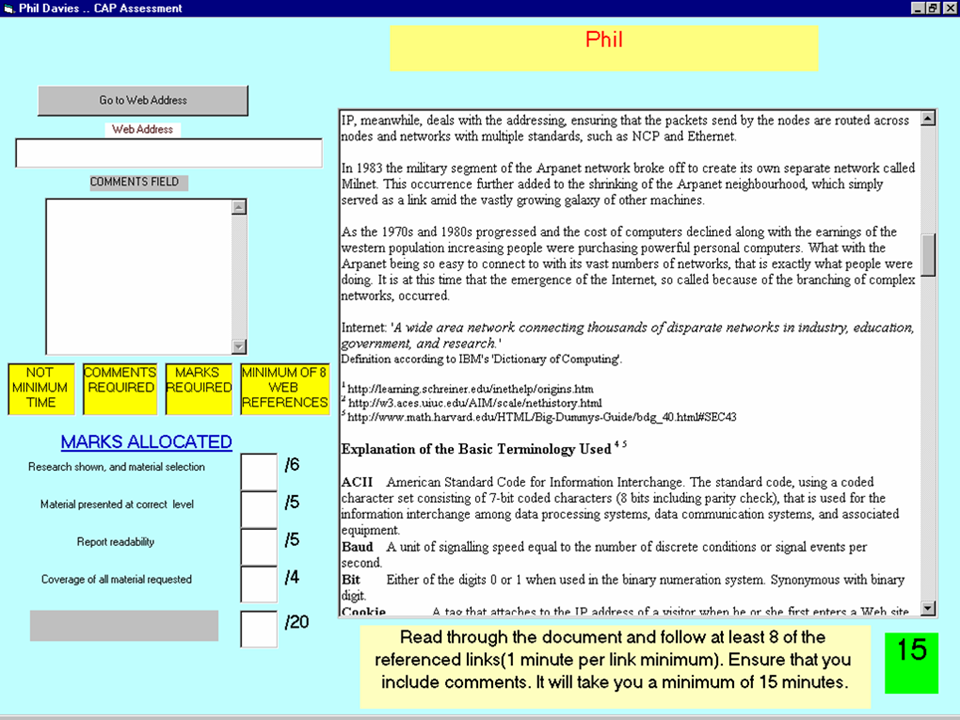
\includegraphics[width=0.8\textwidth]{fig/CAP.png}
\caption{\footnotesize The CAP system, showing report viewer, marking instructions and comment field in its feedback view}
\label{fig:cap}
\end{figure}


In the 1990s, the University of Nottingham produced Ceilidh, a system that had the intent of automating and improving the assessment process for C Language Coursework. Later improvements were made by Heriot-Watt University adding support for
Standard ML (SML) \cite{foubister_automatic_1997}. This tool was used to guide students through the coursework, and then check the correctness of submissions. Ceilidh offered a skeleton answer to students, which pointed out any special language features that should be used. The submitted solutions are checked for correctness with a mixture of verifying output against a model solution, and checking the style of the code (e.g line count, use of certain function names, etc).  In particular for SML, students were asked to provide the types for written functions, as an additional test of understanding.\par
A study conducted by Foubister et al. investigated if such a system used for automatic assessment of students would be useful. To check this, the results of the final exam mark were compared to those marks from previous years where Ceilidh was not used. The study found that there was no real improvement made by Ceilidh, but most importantly there were no detrimental effects. Some positive side effects were observed: The time taken for students to receive feedback on the coursework was markedly decreased, and the tracking of progress offered by the tool allowed teachers to more easily identify any students that were having serious difficulties.\par
Given that I wish to implement a system that is more geared towards peer assessment rather than automated assessment, I think that the most valuable idea to draw from this would be the tracking that is offered to the teacher. Even though it is the students who will be doing the actual assessment, teachers should be able to see how students are progressing with these.\par

In 2002, M. Goldwasser started a peer testing initiative on a Data Structures course \cite{goldwasser_gimmick_2002}.  The main objective of this was to get students taking the course to submit, along with coursework, a test case to run on the program with the aim of finding bugs in other students programs. The main objective in this case was to focus learning on software testing, and the peer testing aspect was secondary, however the study does hold many parallels with my intended system design.\par
The submitted coursework solutions would be collected, along with each test case. Then, using an automated system each of the test cases would be run against each of the solutions. The major downside to this being that there is $x^2$ complexity in terms of the submission count.\par
Goldwasser offers some advice for potential future implementations of such an automated testing system:
\begin{itemize}
 \item To prevent some students falling behind due to having buggy input parsers, have the lecturer provide a standard implementation to to all students. Similarly, output needs to be handled in a standardised way.
 \item A limit should be placed on how large a test case a student can submit.
 \item The automated testing system should be able to handle the case where a solution works correctly, produces the wrong output, crashes, or does not terminate.
 \item Additionally, the testing system should be able to recover and restart from a given position without having to re-run all test cases, or re-run specific test cases if one of the submissions should change
\end{itemize}
I believe this advice is quite useful for our purposes. If building such a system, it is worthwhile to know and consider the various states a program could exit with when running the tests cases. This is still useful even if the implementation I create does not perform a full running of each test to each solution. The suggestion that the lecturer provide a way to handle input and output in a standard way is useful, but more so for lecturers who will set coursework assignments for the website.\par
Additionally, Goldwasser left the autograder used within his study open for download \cite{goldwasser_autograde_2002}. This script could be used as a starting point for implementation of running test cases. However, it does seem to offer more than I require, such as automatically grading (beyond just verifying test cases), and checking against a model answer.

\subsection{Contest Platforms}
As an aside to peer assessment, one optional feature of such an implementation could be to offer automated testing. If a lecturer so wished, they could use the system with a pre-submitted test case. In effect, acting as a peer to each student, so that they could receive test results immediately (or as quickly as the test completes) upon submission.\par
The effectiveness of an automated testing tool (as a sole means of feedback, outside peer assessment) was investigated Farnqvist \& Heintz \cite{farnqvist_competition_2016} within a Data Structures Course.\par
This study investigated how introducing a competitive element to a Data Structures and Algorithms CS course might help students to learn. The survey took place over two runs of the course over 2011 and 2012. In the 2011 course, lab contests were graded manually, and a voluntary contest used an automated grader. In the 2012 course, the lab assignments were marked using an automated grader for testing correctness and efficiency, and by human lab assistants to check code quality. The automated grader in use was \textit{Kattis} \cite{enstrom_five_2011}\par
This test showed the attitudes of some students towards the use of an automated grader. Students found this automated grading to be more fair than the manual equivalent. The study also found that ``students put in more effort in the course thanks to automated assessment''. This would suggest that allowing my implementation to be configured to run as an automated tester might be a worthwhile addition.\par
For the competitive element of this, the study found that competition positively affected student behaviour. The element that was most useful for the contest aspect of this was the autograder. The automated marking and tracking of marks proved useful in motivating students, by offering a leaderboard.\par


Build-it, Break-it, Fix-it\cite{ruef_build_2016} is a programming contest that uses the concept of a Peer testing system to judge the success of various programming assignments. This success is measured both in terms of general correctness and specifically in the context of security. This is somewhat different to the aim of an educational peer assessment website, however it is worth mentioning as the implementation used by the project is, I believe, a good starting model for my implementation of a web platform.\par
\begin{figure}[ht]
\centering
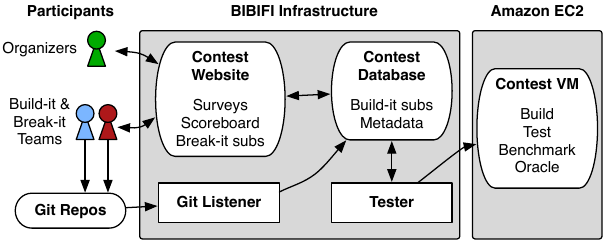
\includegraphics[width=0.9\textwidth]{fig/bibifi.png}
\caption{\footnotesize Basic diagram showing the architecture of the BiBiFi contest system.}
\label{fig:bibifi}
\end{figure}
The contest requires participants to \textit{build} a working solution that matches functional specifications, as well as being as secure as possible. If the solution can be built and the functionality verified by an automated system, then the team can move on to the next stage. Following this, testers will attempt to \textit{break} the security of the solution, and points will be allocated according to a zero-sum-game. The builders can then gain points by \textit{fixing} their solutions.\par
Throughout the contest, there is a central web-based infrastructure that manages running the contest website (with scoreboards, etc.), listening to builder git repositories, and also running and recording test results. The basic structure is as follows (detailed in figure \ref{fig:bibifi} \todo{ref properly}:
\begin{enumerate}
 \item There is a listener component that tracks changes to the git repo of the builders
 \item This pulls metadata to the contest database
 \item The database can activate and get results from the tester component
 \item The tester can use Amazon EC2 to create virtual machines which run the solution, and the tests, then check the results against a benchmark and oracle to see if all is correct (or not)
 \item After reporting this back through the tester to the database, the website front end will update any scoreboards
\end{enumerate}
The basic architecture described here seems to work very well for the contest, and I believe with some modification would be a good starting point for my own implementation. There is no need for git repositories, as the files are uploaded directly to the system. This could just represent the servers file system. Also, while a VM creation system might work well for the contest, I feel that this might be too costly, in monetary terms and time overhead. A simpler sandboxing solution might make more sense, particularly if the system is password protected and only used by students who probably don't want to risk losing coursework marks. (Additional security measures are discussed in \S 1.3.2).

\subsection{Summary of Tech-Enhanced Platforms}
There are many advantages, with respect to learning, brought forward by technology enhanced platforms. Some, such as web-based VLEs are more accessible, allowing students to take part in collaborative exercises from outwith the time and space constraints of a classroom. In Computer Science classrooms, technology is often used to aid in the automation of program testing. This can have positive effects such as giving quicker feedback on solutions and more accurately checking the correctness of solutions with many inputs. These tools could also provide more feedback to the teacher of a class, such as the progress being made by students, to help identify any problems. These systems can also be useful in contests, outwith classrooms and within. Within classrooms, contests using such systems can encourage students to perform better. Such systems can also evoke ideas for how a new technology enhanced learning system could be implemented. This includes the style of architecture, the interfaces that could be used and the general flow of the applications in use.\par



% END
% IMPLEMENTATION BACKGROUND
% BEGIN

\section{Implementation Considerations}
From the previous sections I can see that there is definitely a space for a website to aid in peer testing code. However, there are many issues to consider when choosing how the website should be developed and implemented.

\subsection{Anonymity}
One issue that can arise when students are interacting with each other from a perspective of evaluating each other is their anonymity. During a peer assessment / automated testing experiment performed by Sitthiworachart et al. \cite{sitthiworachart_effective_2004}, the students remarked about the use of anonymity. One students response suggested that in a non-anonymous peer assessment exercise, their marking would be influenced if they knew who it was they were marking. Another student said they would decline to take part if the peer assessment was not conducted anonymously. What can be drawn from these comments is that anonymity is clearly very important to those taking part in the peer assessment. But the opinions of anonymity might not correlate with the actual effect it has.\par

To study the effect that anonymity has, as opposed to just opinions about it, a study was conducted by Lan Li \cite{li_role_2016}. This study aimed to investigate just how effective anonymity is when it comes to making peer assessment more effective, and whether any negative impact from a lack of anonymity can be mitigated.\par
This quasi-experimental study was conducted with some in-training teachers, and aimed to see which is the most effective method of / using / while conducting a peer assessment exercise: Having assessors and assessees know each others identities, remain anonymous, or know identities while having received training. The training in this case involved watching a video that described some of the stresses and concerns that arise during peer assessment, and various forms of discussion regarding this.\par
One issue I have with this study is that it didn't cover the case of being anonymous and getting training. This was because the training was intended as a fallback for when anonymity is not possible. But this does invite the question of just how effective would anonymity be if training were offered as well.\par
The study found:
\begin{enumerate}
 \item ``Anonymity improves student performance in peer assessment''
 \item If anonymity can't be guaranteed, negative effects arising from this can be offset using training
 \item Anonymity does not reduce the pressure and tension related with peer assessment
\end{enumerate} 

From the evidence available, I can gather that there is a great importance in creating a peer assessment system which can function while maintaining anonymity. It might also be worthwhile integrating some form of training, as found in the study by Lan Li, as this might reduce stress during the peer assessment process, as it is not outwith the real of possibility that students might recognise the work of others even if it is anonymous.

\subsection{Security \& Sandboxing}
If the website I aim to create is going to integrate built-in running of test cases I will need to make sure to use the right way of doing this. Because the website I aim to build will accept solutions from students that will need to be executed, it is important that these applications be restricted in terms of the permissions available to them. Restricting how they can interact with the executing computer will prevent malicious attacks or accidental errors in code from damaging the whole system.\par
Some available security measures include AppArmor, SELinux, FBAC amongst others. A study by Schreuders \cite{schreuders_empowering_2011} investigated how easy it is to set up the relevant security measures. They found that the FBAC-LSM security model was the best in terms of the ease of setting up, and ensuring that programs worked correctly. The tool offered for FBAC-LSM security set up would be a good candidate for use in a peer assessment system for running programs.\par
There is also the idea of running programs directly in a browser, using a JavaScript interpreter in a way such as PyPy.js \cite{pypy.js_web_2016}. In this manner, the local file system would be protected, as the file system used by the python interpreter is virtual in memory. However this would not be an ideal solution, as if there were security risks they would simply be placed upon the assessor instead. Additionally, this model of execution would make it more difficult to get and store results of tests and would need to be run synchronously in the website UI. Long operations also block the browser from functioning (having tried this myself, I can see that this would be an issue).\par
Another method might be to modify source codes to use a language-specific sandboxing features. One example of such an interpreter/compiler is PyPy\cite{pypy_pypy_2016}, which is designed to offer some sandboxing. However, this is still in development and could not be relied upon for our purposes.\par
One issue with sandboxing security mechanisms is that such systems can only protect the system by blocking access certain API calls. To put it another way, sandboxes cannot in and of themselves identify malicious code. For this reason it might be worth integrating some form of anti-malware analysis as well.\par
As an alternative to sandboxing, one common method is to re-map the root directory to prevent an application from accessing files on the system that it should not. This is known as a chroot jail \cite{ubuntu_basic_2016}. This could be a useful way of restricting the solution submitted so that it can only access relevant files.

\subsection{Testing Submitted Solutions}
When considering the testing of software, there are several ways that this can be done. To produce a website that enables peer assessment, an appropriate testing methodology will need to be selected. Based on suggested testing styles from Bill Laboon \cite{laboon_friendly_2016}, some testing methodologies were considered for inclusion:
\begin{itemize}
 \item Linting - Performing basic checks for 'smells' of bad code design, such as identifying unused variables or methods. Not particularly useful from a perspective of checking code is correct, but is still useful in terms of producing good quality code.
 \item Unit testing - The use of xUnit style tests. Often used in test-driven development, these could be useful in detecting flaws if written post-development by a peer assessor. This would need the assessor to be familiar with how to write xUnit style tests, and how they should be structured, or it would not be viable.
 \item Expected output testing - Running a program with some input and comparing the output to what is expected. The issue here is that the peer assessor first needs to know what the correct output is. Unlike unit testing, this would simply involve a series of inputs, and a series of expected outputs, and the task of checking the correctness from these tests is left to the website.
 \item Scenario Testing - Simulate an actual usage scenario. Assessors would use solutions as if they were 3rd party libraries (a 'black box'), and develop their own programs that would use these as if in an actual use case. These programs would perform checks to make sure the solutions being tested were running as expected. This is more involved than unit or expected output testing, as it might be better placed to discover side effects of continued use of the solution.
 \item Property based testing - Using a proof checker, such as QuickCheck (or a similar implementation for languages other than Haskell) to ensure that a program is acting correctly. This would place additional overhead onto the students as assessors, as they would need to learn and understand the annotations used by a proof checker, but could provide a lot of coverage of possible inputs.
\end{itemize}
In all cases, the solution being tested needs to conform to a standard interface. And in each case, the website running the tests needs to be able to extract some meaningful information. This is simpler in terms of unit and expected output, as these will offer output that will be easily readable (e.g. by diff, a count of pass/fail tests); scenario and property based tests would produce more verbose output, which while may be more informative, would be harder to analyse and subsequently summarise. 

\subsection{Recording Feedback}
In addition to recording the results of test cases, to enable full peer assessment beyond just peer testing, the desired website should integrate methods of providing feedback through testers critical evaluation of solutions. There are many different ways this could be achieved however, beyond just receiving and recording a paragraph or two of text from the tester.
\subsubsection*{Inline Code Annotations}
One feature seen in Agile software development cycles is the Code Review \cite{github_project_2016}. This involves a colleague reviewing new code, and leaving comments for improvements. GitHub enhances this process by offering inline code annotations. These allow for feedback to be more targeted and, from this, likely easier to understand. This could be a useful feature to implement, as student testers could leave comments for the developers where necessary in the code.
\subsubsection*{Marking Against Criteria} 
To once again draw on research conducted by Falchikov \cite{falchikov_improving_2013}, they discuss peer assessment traits in terms of the criteria used to mark other students. There are different levels of input that students can receive while engaging in preparations for peer assessments. The teacher may provide all of the criteria for marking/assessing; there may be discussion between the students and teachers, where each decide what criteria are important; and lastly offering full control of the criteria to mark over to students. In an open ended answer situation, as is offered by programming exercises, this may be a good environment to encourage the student to come up with more of the criteria.\par
Given a criteria to mark against, it would be useful to integrate some simple systems to check that a given solution meets the defined criteria. Falchikov describes that some common methods used are Likert scales or checklists, working against a known criteria.

\subsection{Summary of Implementation Considerations}
Given the many different aspects covered above, I have identified the following key considerations when implementing the website:
\begin{itemize}
 \item A desirable outcome would be to have a website that can operate without any students knowing the identities of the students whose code they are testing and assessing.
 \item It will be important to impose some form of security on the website. There are many measures that could be taken here, including sandboxing mechanisms, that is restricting the operating system access of the executable; running an executable in a more secured environment, such as a jail; or including malware detection software.
 \item There is a choice of methods to employ when creating test cases. The test cases testers will write could include linting, unit testing and scenario testing, amongst others.
 \item Feedback could be collected from the testers through free comment in various places of the application, or by checking against a marking criteria.
\end{itemize}

% END

% SIR GLOSSARYCK, OF TERMS
% BEGIN
\chapter{Glossary of Terms}
The following is a glossary of terms used in the remainder of this dissertation. It is provided to consolidate some points made in the background research chapter and to make clear some terms that will be used later on, to prevent confusion.\\
\gloss{Feedback}{Following a peer assessment, feedback is given to the testee indicating how good the solution found was\todo{not good definition}}
\gloss{Oracle}{A solution that offers a known-to-be correct implementation students can run their test cases against (although it will not be visible to them}
\gloss{Peer Assessment}{The process of reviewing an assignment where the students assess each others work (in whole or in part), and the results of this may be further used in grading assignments.}
\gloss{Peer-Testing}{A subset of peer assessment, in which students test each others programming code}
\gloss{Signature Test}{This is a test case designed to ensure that the student has met the interface that was described to them}
\gloss{Solution}{A solution to a coursework assignment, possibly written by a student}
\gloss{Submission}{A solution, test case, coursework descriptor, etc. Any item made up of one or more files that is uploaded to the system by a student or teacher.}
\gloss{Test Case}{A students test case that is to be run against a solution}
\gloss{Test Match}{A matching of a test case and a solution. It will eventually have results, and may also have attached feedback}
\gloss{Website}{Shortened form referring to a web platform or web application}
% END


% objectives
% BEGIN
\chapter{Objectives}
\section{Primary Aim}
The primary motivation of this project, as stated in the introduction, is to improve the student experience when completing programming coursework exercises by facilitating peer learning. The main aims for the project derived from this can be stated as:
\begin{enumerate}
\item \textbf{Prototype a Website}\par
Design and build a website that automates peer assessment, with a focus on peer-testing. This website should combine all the tasks that would normally have to be done manually by students and allows them to be completed from a website interface. This could include file uploads, file viewing, testing of programs and providing feedback. The objectives for the Prototype are broken down further in section \S4.1 \todo{pop them in here as well, or is that going to repeat too much?}.
\item \textbf{Evaluate the Website}\par
\label{sec:aimeval}
Once a functioning prototype is created, perform a study to determine the effectiveness of the website in terms of how well it enhances peer assessment and peer-testing within the confines of the coursework. This evaluation should involve students who might potentially use this tool in a course. The exact properties I wish to ensure the website has are expanded upon in the evaluation discussion, Chapter 7. Namely, these are to test the Correctness, Usability, and Security of the implementation as well as seeing if this improves the peer-testing process by giving Enhanced Feedback, and improves the Speed of turnaround of testing.
\end{enumerate}

\section{High Level Objectives}
To further break down these aims, I wish for the project to meet the following objectives:
\begin{itemize}
\item Create a website
\item Let developers submit solutions to website
\item Let testers run test cases against solutions
\item Let testers give feedback on the solutions
\item Report this feedback / results of tests to developers
\item Test the website to make sure it is free of bugs
\item Test the website to make sure it is useful for peer assessment through peer-testing
\end{itemize}
%END


% 1st iteration
% BEGIN
% Work testing various technologies
% Initial bits of implementation
% Refining a working single-file prototype
\chapter{Initial Prototype}
Following the completion of the background researched, the next step of the project was to develop an initial prototype, to test that the concept could actually be built and tested. This would require identifying and choosing suitable technologies, designing an interface and designing and implementing a system.

\section{Prototype Objectives}
\todo{may want to trim this as needed - want to be relevant to initial prototype only}
\todo{the \S numberings will all be wrong}
These are the objectives that relate to the Prototyping of the peer testing website. These are further broken down into requirements in the next section on implementation (\S4.2).
\objitem{Submit}{File upload for solutions}{High Priority}{The website will let students upload solutions to assignments. The website will also assign this solution to one (or more) other student for assessment.}
\objitem{Test}{Build test cases}{High Priority}{The website will let students build, and subsequently submit test cases in a simple way. As previously discussed in \S1.3.3, possible implementations of this subsystem include many different forms of testing, such as Unit Testing, Property based testing and more.}
\objitem{Run}{Run test cases}{High Priority}{Once the test cases are built, run them. The results of running them will be stored for later display. This is done asynchronously to the main interface, as running the test cases may take some time. This could extend to running a submitted test against all solutions.}
\objitem{View}{Viewing own solution}{High Priority}{Let the student see their own submission, which test cases have been run against it, the status of each test, any feedback from peer assessors.}
\objitem{Results}{Display test results}{High Priority}{Display the results of a test against a particular solution. Display the results (passed, failed, error, metadata) on each test.}
\objitem{Security}{Secure the System}{Medium Priority}{As the website acts as an open interface for running python, it is important that it be secured against attacks (malicious or accidental), and that only the relevant people may access it.\par
While in a production system, security would normally hold a high priority, in this prototype stage, the focus will be more so on the functionality that evaluation test subjects will interact with. Given that this evaluation will be monitored, test subjects can be prevented from uploading malicious code. However, this prototype will need to have some form of authentication in place, to make sure that only developers and test subjects may access the website.}
\objitem{Feedback}{Provide feedback on solution}{Medium Priority}{A tester should be able to provide feedback to the developer at various stages of the assessment. This could include at the results of tests or on the source code.\par
An ideal implementation of this would provide a way for testers to give feedback to the solutions, within certain places of the peer assessment \todo{... what?}. Possible objectives that could interact with feedback include:
\begin{itemize}
 \item OBJ-Results: Once tests are run, the tester could attach comments to the (results of) test cases
 \item OBJ-Source: Annotating the source code of solutions (possibly on a line by line basis, or by leaving general comments for a submitted solution)
 \item OBJ-Teacher: A teacher should be able to view all of the feedback that has been submitted by testers, in all the appropriate places
\end{itemize}~}
\objitem{Source}{Show source code}{Medium Priority}{A tester should be able to read the source code of a solution, for example to inspect the coding style (variable names, structure etc.)}
\objitem{Teacher}{Teacher overview screen}{Low Priority}{Provide a way for the teacher of the class to set the coursework. Also, to see all of the solutions and the tests run on each of them, as well as any feedback.}
\objitem{Modular}{Create a modular system}{Low Priority}{One motivation for building the system would be to plug it into other learning tools, such as Moodle.}
\objitem{Record}{Record metadata about run solutions}{Low Priority}{When running solutions with test cases, record metadata such as time taken to complete, memory usage, code coverage, etc. Store this data for display with each test result.}

\section{Initial Prototype Requirements}
Based on the  prototype objectives previously outlined (\S4.1), I can establish the following system requirements:\par
The following prioritisation is used: \textbf{Low} - Possible future addition, \textbf{Mid} - Would make a more useful system, \textbf{High} - Necessary for prototype.
I also detail which of the requirements I was able to complete in this first iteration, denoted by a $\bigtriangleup$.
\begin{longtable}{cclrc}
\textbf{ID} & \textbf{Objective} & \textbf{Description} & \textbf{Priority} & \textbf{*} \\\hline
\freq{Security}{Log students in}{High}{$\bigtriangleup$}
\freq{Security}{Log teachers in}{Low}{$\bigtriangleup$}
\freq{Submit}{Accept student uploads of solutions to assignments}{High}{$\bigtriangleup$}
\freq{Submit}{Assign a submission to a student for assessment}{High}{$\bigtriangleup$}
\freq{Test}{Accept uploads for test case files}{High}{$\bigtriangleup$}
\freq{Test}{Offer a more guided approach to writing test cases}{Mid}{}
\freq{Run}{Run submitted test case for the submitted solution}{High}{$\bigtriangleup$}
\freq{Run}{Record the results of test execution}{High}{$\bigtriangleup$}
\freq{Run}{Run submitted test case against all solutions}{Low}{}
\freq{View}{List all test case submitted}{High}{$\bigtriangleup$}
\freq{View}{Display the results of running a test}{High}{$\bigtriangleup$}
\freq{View}{Display the results of all solutions test run against}{Low}{}
\freq{Results}{Let submitter of test see the results}{High}{$\bigtriangleup$}
\freq{Source}{Let tester see source code of solution}{Mid}{$\bigtriangleup$}
\freq{Feedback}{Let submitter of test add/edit feedback \todo{move edit as s2 req}}{Mid}{$\bigtriangleup$}
\freq{Feedback}{Record testers general comments on solution}{Mid}{$\bigtriangleup$}
\freq{Feedback}{Let tester attach feedback to lines in solution}{Low}{}
\freq{Security}{Sandbox the execution of solutions}{Mid}{}
\freq{Security}{Use malware detection to prevent malicious uploads}{Mid}{}
\freq{Teacher}{Let teacher set coursework assignments}{Low}{$\bigtriangleup$}
\freq{Teacher}{Let teacher see all submitted content}{Low}{$\bigtriangleup$}
\nfreq{Website}{Operate on Desktop Web Browsers used in classroom}{High}{$\bigtriangleup$}
\nfreq{Website}{Operate with multiple users accessing at once}{High}{$\bigtriangleup$}
\nfreq{Website}{Operate with a classroom of users accessing at once}{Low}{}
\nfreq{Submit}{Not assign a student to assess their own work}{High}{$\bigtriangleup$}
\nfreq{Submit}{Accept solutions that are python scripts}{High}{$\bigtriangleup$}
\nfreq{Run}{Test cases should be run asynchronously}{High}{$\bigtriangleup$}
\nfreq{Modular}{The system should be built in a modular manner}{Low}{$\bigtriangleup$}
\end{longtable}

\subsection{Additional Notes on Requirements}
Regarding requirements which are prioritised as low, this is because for the purposes of our prototype and evaluation, these requirements are not fully necessary. For example, teacher interactions can be hard coded for the evaluation. The main focus at this stage of development is to ensure that the interactions for students who will test the website work as well as possible.

\section{Use Cases}
To better describe and visualise the requirements for the application as a whole, the use cases described in figure \todo{which} (and the included extended descriptions) are given.
\begin{figure}[ht]
\centering
\begin{tikzpicture} 
\begin{umlsystem}[x=0, y=0]{Peer-testing website} 
\umlusecase[y=-2, x=-2]{Authenticate}
\umlusecase[y=-3.5, x=-2]{View Coursework}
\umlusecase[y=-2, x=2, width=2cm]{Create \& Edit Coursework}
\umlusecase[y=-7, x=2, width=2cm]{View, Create \& Edit Course}
\umlusecase[y=-9, x=2, width=2cm]{Create \& Run Test Match}
\umlusecase[y=-5, x=-2]{View Test Match}
\umlusecase[y=-9, x=-2, width=2cm]{Create Test Match Feedback}
\umlusecase[y=-7, x=-2, width=2cm]{Upload submission for coursework}
\end{umlsystem} 
\umlactor[x=-7, y=-6]{student}
\umlactor[x=7, y=-6]{teacher}
\umlassoc{student}{usecase-1}
\umlassoc{student}{usecase-2}
\umlassoc{student}{usecase-6}
\umlassoc{student}{usecase-7}
\umlassoc{student}{usecase-8}
\umlassoc{teacher}{usecase-1}
\umlassoc{teacher}{usecase-2}
\umlassoc{teacher}{usecase-3}
\umlassoc{teacher}{usecase-4}
\umlassoc{teacher}{usecase-5}
\umlassoc{teacher}{usecase-6}
\end{tikzpicture}
\caption{Diagram showing the main use cases implemented at this iteration of development. Both Student and teacher are sub-actors of User}
\label{fig:i1uc}
\end{figure}

\singlespacing
\subsection*{UC - Authenticate}
\textit{A user wants to log in to the website using their credentials - a username and password}\\
\textbf{Primary Actor}: User\\
\textbf{Preconditions}: A user is not already logged in, The user is registered on the website, user is at login web page\\
\textbf{Main Flow}:
\begin{enumerate}[noitemsep,nolistsep]
\item Website requests credentials
\item User submits credentials through a form
\item Website checks that these match expected values
\item \textbf{If not:} Go to step 1
\end{enumerate}
\textbf{Postconditions}: User is logged in, user is at main index page

\subsection*{UC - Create \& Edit Coursework}
\textit{A teacher wants to create a coursework, or update the values of an existing one}\\
\textbf{Primary Actor}: Teacher\\
\textbf{Preconditions}: A teacher is logged in\\
\textbf{Main Flow}:
\begin{enumerate}[noitemsep,nolistsep]
\item Website requests information for coursework
\item Teacher submits details through a form
\item Website updates coursework with these details
\item \textbf{If coursework does not exist:} Coursework is created with these details
\end{enumerate}
\textbf{Postconditions}: Coursework exists with new values, any old values are overwritten

\subsection*{UC - View Coursework}
\textit{A user wishes to see the full details for a coursework, and any files associated with it}\\
\textbf{Primary Actor}: User\\
\textbf{Preconditions}: User is logged in, user is enrolled on the course for a coursework\\
\textbf{Main Flow}:
\begin{enumerate}[noitemsep,nolistsep]
\item User selects a coursework item
\item Website selects the appropriate view for their permission level
\item Website collects information about coursework
\item Website collects files related to coursework that user has permission to view
\end{enumerate}
\textbf{Postconditions}: Website displays coursework details to user

\subsection*{UC - View Test Match}
\textit{A user wishes to see the results of having run a test, and the files that were involved with it}\\
\textbf{Primary Actor}: User\\
\textbf{Preconditions}: User is logged in, user is enrolled on the course for the given test match, test match has been run\\
\textbf{Main Flow}:
\begin{enumerate}[noitemsep,nolistsep]
\item Website checks that user has permission to view test match - i.e. they are a teacher, they created the test match, they are assigned to give feedback on it, etc.
\item Website gathers list of files associated with the test match
\item Website displays those files that user has permission to view
\end{enumerate}
\textbf{Postconditions}: The user is shown everything related to the test match that they have permission to see

\subsection*{UC - View, Create \& Edit Course}
\textit{A user wishes to see details of a course, possibly edit it, or create a new one}\\
\textbf{Primary Actor}: Teacher\\
\textbf{Preconditions}: Teacher is logged in\\
\textbf{Main Flow}:
\begin{enumerate}[noitemsep,nolistsep]
\item Teacher chooses a course
\item Website displays details of course in a form (name, code, enrolled students)
\item \textbf{If creating}: Website displays a blank form
\item Teacher may edit this form and submit it
\item The contents of the form are validated
\item The database is updated
\end{enumerate}
\textbf{Postconditions}: Course is updated, or a new one created, with these details; the teacher is shown the newly updated coursework

\subsection*{UC - Upload submission for coursework}
\textit{A student wants to submitsome sort of answer submission for a coursework - e.g. a solution source code or a test case}\\
\textbf{Primary Actor}: Student\\
\textbf{Preconditions}: Student is logged in, student is enrolled on course, coursework is accepting submissions\\
\textbf{Main Flow}:
\begin{enumerate}[noitemsep,nolistsep]
\item Student picks file(s) for submission, and the type of the file (solution, test case)
\item Student uploads this to website
\item Website Processes this uploaded submission
\end{enumerate}
\textbf{Postconditions}: The submission is uploaded to the website

\subsection*{UC - Create \& Run Test Match}
\textit{A teacher wants to match a solution and a test case together and get the output of running them}\\
\textbf{Primary Actor}: Teacher\\
\textbf{Preconditions}: Teacher is logged in and enrolled on a course\\
\textbf{Main Flow}:
\begin{enumerate}[noitemsep,nolistsep]
\item Teacher views file uploads for a coursework
\item Teacher selects a solution and test case
\item Teacher decides whether to keep it invisible from students, to make it visible to developer, to assign a marker\todo{conflicting wording - tester}
\item Teacher submits these details
\item Website processes this request, creates a test match
\item The test match is queued to run
\end{enumerate}
\textbf{Postconditions}: Depending on the configuration of the website, the test match may be queued to run or run immediately. After it has run the results are stored in a file\\
comment: \todo{this is changed later to allow students to also create test matches..., mention appropriate anonymisation of results - e.g. dirs and paths... have a special method in pipeline of running rsults in code?}

\subsection*{UC - Create Test Match Feedback}
\textit{A student has viewed a test match and wants to give feedback to the developer}\\
\textbf{Primary Actor}: Student\\
\textbf{Preconditions}: Student is logged in, enrolled on course, student has viewed test match\\
\textbf{Main Flow}:
\begin{enumerate}[noitemsep,nolistsep]
\item Student submits feedback text
\item Website stores this as a file
\item Website attaches this file as one related to the test match
\end{enumerate}
\textbf{Postconditions}: Feedback is submitted, next time it is viewed, feedback will be shown as well as other files
comment: \todo{note that the idea of giving feedback just on solutions may be faulty, may want to feedback test cases as well, in addition, mention somewhere about extended interaction / discussions for feedback rather than single  comment. note lack of feedback editing}

\section{Sequence of Operations}
In order to better grasp the sequence of operations that a class of users (student developers, testers, and teachers), I have developed the following sequence diagram. \todo{note that this was improved upon in the next iteration of development}\\
\begin{figure}[ht]

\caption{Sequence diagram showing how students, teacher and the website interact during a coursework exercise}
\label{fig:i1sd}
\end{figure}


\section{Choosing Tools}
There are many ways that the website could be built. To identify some options, I considered the available software on the university servers, and Identified languages and frameworks that could be used here:\par
\textbf{Languages:} Java Server Pages, PHP, Python\par
\textbf{Frameworks:} CakePHP, Django (Python), Flask (Python)\\
I decided it would be beneficial to use a language I was familiar with, to allow me to prototype more rapidly, so I decided to choose between some sort of PHP or Python based option, having had previous experience with these.\par
I considered if it would be better to use a framework or start scripting using raw files but decided it would be better to use a framework, as these often have abstractions that can offer standard security measures (for example, user form input validation), as well as other abstractions to help speed up creation of website applications (such as HTML templating\footnote{This is when you create a static HTML template, and at runtime fill it in with relevant values, enabling better re-use of HTML code}).\par
Given that I would need to restrict the scope of the peer-testing website for this initial prototype I decided, with the suggestion from my supervisor, that it would make sense to use the same language in both the website and the coursework exercises that might be used within the live website, as having the same language features for developing both the website and the method for offering testing might be easier to develop. Such a design would need to be carefully chosen to be modular, as this might increase the temptation to form tightly coupled code.\par
To this end, I have chosen to develop the application using a python web framework. For initial selection of some frameworks, I attempted to develop sites that allowed a user to authenticate themselves with a password. I found that this was much easier to do with Django, as it offered its own middleware for authentication, as well as many other features such as a clear model-view-controller style. Flask on the other hand was much more low level. I did not feel it would be worth spending a lot of time developing low-level web application technology myself, so decided to go with Django.\par
\section{Initial Prototype Development}
For this initial prototype, I would aim to get the core functionality implemented:
\begin{itemize}
\item User Authentication
\item File Uploads and Serving
\item Managing Coursework
\item Running Tests
\end{itemize}
Given that Django offers some prefab content for authentication, this was easily implemented.\par
For file uploads, the main issue was of how to get them from the file and store them on the filesystem. The standard Django methodology for doing this would be to create a form class with the relevant file upload field. Then, within a view, display this form and extract the file for saving through a POST request. Django can then store an uploaded file by instantiating a Model in a database. This process could have perhaps been done using a standard HTTP PUT request, however I felt it would be more secure to use the standard Django method.\par
The file could be written directly to the system, but using the database offers a nice abstraction that means lower level file system management operations are not required. This also simplifies development of finding files later (if not necessarily the actual efficiency of the operation), as you would not have to search through a filesystem, just rows in a database tables.\par

\section{Initial Interface Design}
\doublespacing
Given that the focus of this initial prototype was more concerned with testing that functionality could work, I have decided to place less of a focus on the UI implementation, However I prepared some mock-ups describing the main sections that users logged into the site would see. These mock-ups are included in an appendix \todo{which one, and remember to add it, and keep stage 2 separate, maybe add more comments on each}.
\subsection{(Students) The Coursework Overview}
After selecting a coursework from a list, the students would be displayed a page that contained all of the necessary instructions to complete the coursework, including links to where they could download full descriptors, code samples, etc. This page also offers a link to a page for uploading solutions to the site. This page also displayed links to the feedback view where students would either give or receive feedback.\par
\todo{Display a mock-up of this early view - possibly the powerpoint slides attached somewhere, and then screenshots of what the initial prototype branch looked like in reality}
\subsection{(Students) The Feedback View}
The purpose of the feedback view is to display files to the student who will be testing and giving feedback. These files will include the solution being tested, the test case, and the results of running the test. In addition, there would be a section where either feedback could be given into a web form, or read if it had already been given.
\subsection{(Teachers) Course Editor}
The course editor is a place where a teacher could manage (or create) a course - e.g. the students who were enrolled on it, the name of the course and the course code.
\subsection{(Teachers) Coursework Editor}
This will likely be the most used view for the teacher - it acts as a way to edit (or create) coursework assignments. The view displays any files that have been uploaded, and lists any tests that have been run. It also offers a way to create test matches.

\section{Initial System Design}
Do we want UML diagrams here? At each `iteration of development stage? wherefore?
\begin{figure}[ht]
\centering
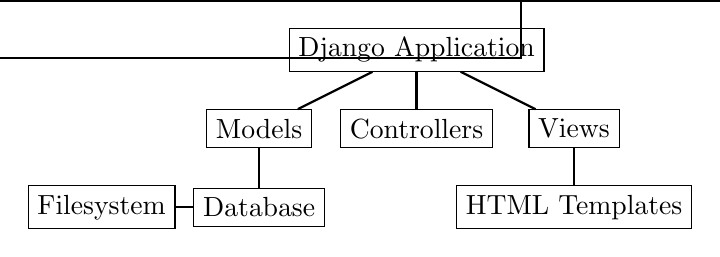
\begin{tikzpicture}
\tikzstyle{box} = [draw, minimum size=10]
\tikzstyle{line} = [thick,>=stealth]
\node (d) [box] {Django Application};
\node (c) [box, below of=d] {Controllers};
\node (m) [box, left of=c, node distance=2cm] {Models};
\node (v) [box, right of=c, node distance=2cm] {Views};
\node (db) [box, below of=m] {Database};
\node (fs) [box, left of=db, node distance=2cm] {Filesystem};
\node (ht) [box, below of=v] {HTML Templates};
\draw [line] (d) -- (m);
\draw [line] (d) -- (v);
\draw [line] (d) -- (c);
\draw [line] (m) -- (db);
\draw [line] (db) -- (fs);
\draw [line] (v) -- (ht);
\end{tikzpicture}
\caption{Diagram showing the main components of the system at this iteration}
\label{fig:i1sysd}
\end{figure}
The initial system uses an MVC style architecture, as is recommended by Django.
\subsection{Models}
The models are defined as Django model classes and then Django automatically implements them in a database. One advantage of creating the models this way is that different database technologies can be switched out. for the prototyping stage, a basic sqlite database was used, that acts as a lightweight database stored in a single file, making it easier to manage during development. This could be switched out to use a dedicated MySQL database when implementation is complete. This method also makes it easier to access data from the database in a object oriented manner, which reduces the reliance on SQL commands for extracting information, and also allows for Django abstractions to offer some performance improvements. One such improvement is by storing queries in a QuerySet object, which can be passed around in code, the database query is executed on-demand which means \todo{finish this thought, make a nicer sentence structure}.\par
Something something files on a filesystem \todo{am i repeating myself?}
\todo{Remember to explain why each choice was made that way.}
\subsection{Controllers}
When a user makes a request to 

\subsection{Views}
In a Django application, the views are instantiated by the controller classes. These take the form of HTML templates, with information filled in at runtime. These support inheritance, which is useful, as it allows for a single template to be created that acts as a base for all part of the website... \todo{et.c. etc.}.\par
Django also offers some standard HTTP responses that can be sent instead of the HTML templates, making it easy to support standard web request-response dialogue, such as informing a user they do not have sufficient permissions through a HTTP 403 Response View.

\section{Notifications}
As part of this initial prototype (but not included in later iterations), was a test of WebSocket-based notifications. These are an example of a Server-Push architecture, as opposed to the regular Client-Server architecture the rest of the site uses. Under server push, a client subscribes to a web socket, and the server may send out notifications. For the purpose of the site, the end product would ``push'' a notification to a user for certain events, such as a new piece of feedback that was received. This would give the website a more dynamic feel.\par
The initial prototype for this offered a simple way to connect to the server, to test if it would be feasible or not. While it was possible to set this up it required additional tools, such as switching from a WSGI web interface to an ASGI interface.\todo{repeating future work? leave it here? mention why it was removed here?}
% END

% 2nd iteration
% BEGIN
% [multi-file, improved test matching plugins, prep for pipeline]
\chapter{Second Iteration Development}
Once the initial prototype was created, I attended a course of two meetings with members of university staff in Edinburgh and Dubai who were interested in potentially using this peer-testing website.\par
\section{Discussions with Stakeholders}
The purpose of these meetings was to further refine what might be required for a full implementation of the website. These were quite insightful, and I have developed the following \todo{notes? changes? requirements?} as a result, including some uncompleted requirements from the initial prototype (marked with a $\succ$), and those that I have completed in this iteration are marked with a $\bigtriangleup$:
\begin{longtable}{cclrc}
\textbf{ID} & \textbf{Objective} & \textbf{Description} & \textbf{Priority} & \textbf{*}\\\hline
\freq{Security}{Log students in}{High}{$\succ$}
\end{longtable}

\section{Modifications to system design}
One of the requests suggested that it would be beneficial to allow multiple files to be part of a single solution or test case - this would be a definite requirement if additional languages are supported beyond python - e.g. languages like C that require separate header files. I have modified the models accordingly. This is the current working layout:
\todo{add a database er diagram thingy}
\todo{somethign something pipeline, originals folder, process inputs, modularity, python and other languages}

\section{Modifications to interface design}
As will be used within an evaluation study, more effort is placed into the design of the UI at this stage than the previous one. Most of the design stayed the same, but in some places it was improved:\par
The \textit{feedback view} was changed to support multiple files being used per solution / test case. Instead of panels with files, there is a tab control that allows the user to switch between each of the files individually. A compromise that only allows one file to be viewed at once, but allows for multiple files to be seen without needing to change/reload the web page.\par
Within the \textit{Coursework Overview}, to encourage students to familiarise themselves with how the system works\todo{a la joe wells suggestion}, they are offered the ability to create their own tests on the system, whereas previously any testing of their own would need to happen offline. This allows them to create a test match, and also lets them access the signature test and oracle. In a similar vein, to encourage additional testing, once students have been assigned someone elses work to test, they can upload additional tests to use when providing feedback.\par
Given the ease with which HTML can be modified, and that much of what I needed was already present, I simply made the UI changes directly without preparing mock-ups. \todo{attach screenshots / appdx}\par
To increase the level of anonyhmity everything public facing was given \todo{random slugs - anon, security etc.}
\section{Further development}
As part of supporting multiple files per submission
\begin{itemize}
\item Setting one submission as final
\item Setting submissions as private
\item ...
\end{itemize}

\section{Live Hosting}
In order to prepare for a live test of the system, I identified some possible options that could be used to host the Django application:
\begin{enumerate}
\item Running the website from a private server
\item Running the website in local debug mode from one of the university machines
\item Running the website on the university Apache web server
\end{enumerate}
For the intended purpose of the website, that it would be used in an educational environment, the most obvious option would be 3. This way, we could ensure that all of the student-uploaded data is kept inside the university ecosystem.\par
While discussing this setup with the University MACS administrators, it was found that in order to run the application on the Apache server either some packages would need to be upgraded or rebuilt, or the Django application would need to be modified to use an older version of Django and python. The latter was not possible, to while the MACS IT team investigated ways to upgrade the server, I worked with my Project Supervisor to host it in a private location.\par
When the Django application was hosted as a daemon process within Apache under WSGI (Web Server Gateway Interface), the requests on a given URL path are routed to the Django application rather than the usual routing to static HTML / PHP scripts. This meant that some modification was needed for the Django application's configuration as errors in serving the website highlighted places where  hard-coded URLs had broken, where relative paths were incorrectly used and where the Apache Linux user did not have the correct permissions to operate on the application. These required relatively simple fixes.\par
The MACS IT team was able to upgrade the required packages such that Apache could operate. Using the changes made for running on the private server as a base, setting up the Django application to run on the university server was easily possible.
% END

% EVAL
% BEGIN
\chapter{Evaluation Study}
\section{Methodology}
In order to conduct the evaluation study I aimed to test the live system with participants pretending to be students completing coursework. Ideally we would have two groups -- one doing the peer-testing using the website and one not. For this study, the participants that were not using the website would be communicating via email.\par
To try and get as fair a response as possible, each participant in each group would complete two tasks, but the pairing of which task would be completed using the website or by email would be swapped between each group. Examples of the tasks that would be completed are given in appendix E (p\pageref{app:descriptors}).\par
Participants filled out a consent form, as can be seen in appendix B (p\pageref{app:consent}), then took part in the peer-testing exercises. Upon completing this, they were given a survey, appendix C (p\pageref{app:survey}) to complete and an invitation to a discussion session, appendix D (p\pageref{app:discussion}). Finally, participants were rewarded with a gift voucher.

\section{Participation}
During the study I had planned for a group of 16 people participating, however throughout the process a lower number, actually took part, with 2 participants withdrawing, and not all participants completing the peer-testing exercise. Overall, 12 used the website at some point and 11 people filled out the final survey.\par
As part of the final survey participants were requested to fill out, the following demographic data was found:
\begin{itemize}
\item The majority of participants were Computer Systems students, with 8 participants. Then, 2 Software Engineering students and 1 Computer Science student.\footnote{Before 4th year, both the Software Engineers and Computer Scientists follow the same course.}
\item Most of those who took part were Year 2 students (7 in total), and 3 from Year 3\footnote{1 Participant did not identify which year they were from}. 
\item There was a decent mix of students from both campuses, with 5 participants from the campus in Edinburgh and 6 in Dubai.
\item There were more male participants, with 7 identifying as male, and 4 identifying as female.
\end{itemize}
I feel that the spread of students that ended up taking part does provide a useful range over the demographics within the university as a whole.
\subsection{Response to the Exercises}
As part of the final survey participants filled out, they were asked their opinions on the tasks they were asked to perform. This section asked participants how well they felt they did on each exercise by asking them to select choices from a set of statements. There was also some space for user input.\par
The \textit{Quicksort} exercise was found, overall, to be easy, likely because many people had completed this exercise before, and that the instructions for the exercise were good. The participants found it enjoyable and easy to write tests for this exercise (both to test themselves and others), and they felt that unit testing was an appropriate method of testing.\par
The \textit{Binary Tree} exercise was found to be challenging by some and easy by others. Some had completed such a task previously, and the instructions were found to be good. Most participants felt it was easy to write tests for themselves and others, and that unit testing was an appropriate method for this task.\par
Overall, I would take these results to suggest that the exercises were well explained to participants, and that the chosen exercises were a good fit for the study as a whole, as they offered a wide range of possible solutions and therefore test case creation. For example, within the binary tree I saw several different patterns of object oriented solutions, and in the quicksort there were a wide variety of ways that arrays were split up for recursion.\par
Questions asked in the discussion session seem to agree with these responses. The students said that they enjoyed taking part, and that the well defined expected behaviours of the tasks made it easy to test. Beyond this, some interesting points were raised regarding the way the tasks were distributed: While there was enough information provided in the various documents for the study, it may have been easier to understand if they had been placed in a single PDF, and that some sort of live/video demonstration would have helped explain the task better.\par
Regarding the solutions that were submitted, there seems to be a great deal of variety - this is good. It shows that the interface was clear enough to follow, but not overly restrictive regarding what people were able to use. The different implementations will hopefully allow those doing the peer-testing to learn by see alternative ways of completing the task\par

\section*{Results}
The following sections will break down the feedback I have received from participants into the major sections that I wished to evaluate, as set out in \S \ref{sec:aimeval}.

\section{Correctness}
\textit{Was the website behaving correctly? Were there any bugs?}\par
\subsection{Failing Tests}
Points raised in the survey suggested that the participants were put off by the number of failing test cases.  Multiple respondents felt that the failing tests limited  their ability to provide meaningful feedback. I include here a list of reasons why tests failed (there were a total of 49 tests):
\begin{itemize}
\item 21 Test Runs completed successfully
\item 12 Runs failed dues to inconsistencies in Indentation\footnote{In Python, indentation is not just code style, but an integral part of the language syntax}
\item 7 Test runs failed due to the implementation not following the spec
\item 5 Test runs failed due to incorrect object oriented programming calls (e.g. trying to evaluate .Right on an object where it was not defined)
\item 3 failed due to the unit tests being written in such a way that they were executable scripts than were run when loaded as unit testing modules
\item 1 Failed due to hitting the recursion limit
\end{itemize}
Another interesting analysis based on the failing tests is comparing the tests written by a tester when run against the testers own solution, and those tests run against another developers solution.
\begin{itemize}
\item Run Against self: 19 Passes, 10 Failures
\item Run Against someone else: 2 Passes, 18 Failures
\end{itemize}
This would suggest that people are making assumptions about each others code, some correct (such as assuming the other developer would follow the interface), and some incorrect (such as assuming they would structure their code in a certain way). Additionally, it suggests that not all of the participants properly tested their code on the site to make sure their indentation was correct. I noticed one participant did indeed re-upload submissions several times trying to correct issues with indentation.\par
As a point of interest, during the discussion session, I asked participants how they feel about python's indentation and this revealed that participants in Dubai leaned more towards Tab-based indentation, and in Edinburgh towards spaces. Another issue raised was that in Dubai the primary development OS is Windows (and therefore the CR-LF line endings), versus Linux used in Edinburgh. These consistencies would cause further issues if someone were to try to change the files during testing. To quote of of the participants - ``Python's a mess''.
\subsection{Permission Issues}
Additionally, one respondent raised the issue that they were unable to see the files of the person they were supposed to be testing. While investigating this I discovered that the issue lay in that the developer had set their solution to be private, which meant that the tester would not be able to see files relating to it. I believe this to be an issue related to usability, which I discuss in section \S\ref{sec:permiss}.

\section{Usability}
\textit{How usable was the website, from the perspective of the end users?}\par
\subsection{General Feedback Given}
To get a quick feel for how usable the site was, I asked some questions in the survey. These were in the form of likert scales (fig \ref{fig:likert-use}).\par
\begin{figure}[ht]
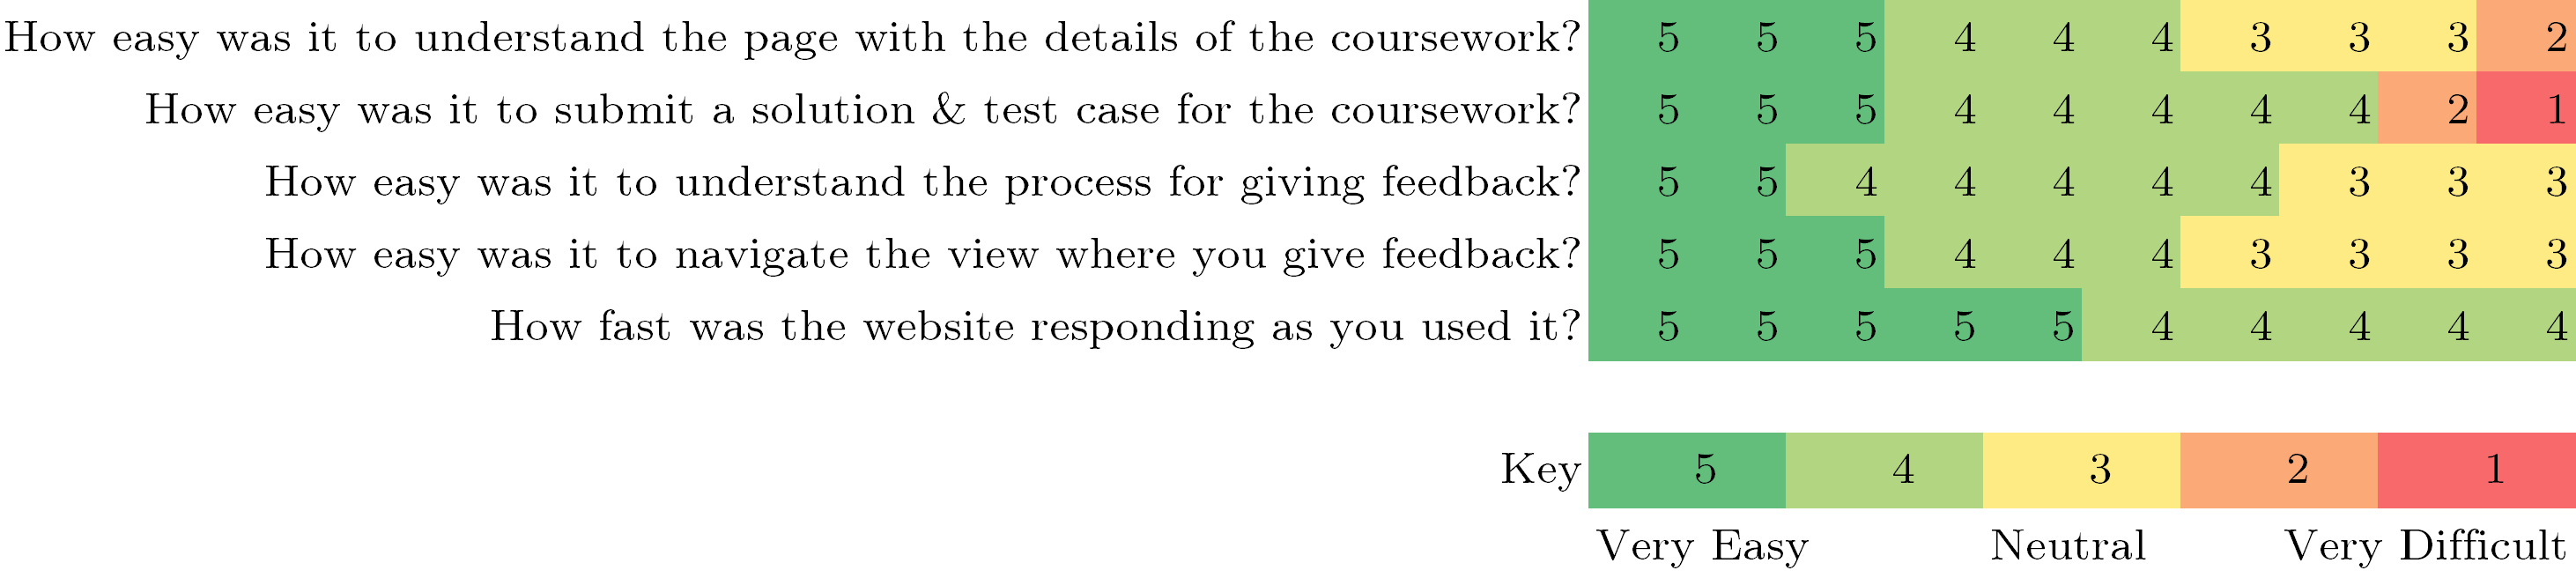
\includegraphics[width=\textwidth]{eva-result/likert-site-usable.png}
\scriptsize
\begin{tabular}{r|lllllllllll}
How easy was it to understand the page with the details of the coursework?  & \cellcolor{Green} 5   & \cellcolor{Green} 5   & \cellcolor{Green} 5   & \cellcolor{LimeGreen} 4   & \cellcolor{LimeGreen} 4   & \cellcolor{LimeGreen} 4   & \cellcolor{Goldenrod} 3   & \cellcolor{Goldenrod} 3   & \cellcolor{Goldenrod} 3   & \cellcolor{YellowOrange} 2   & \cellcolor{YellowOrange} 2\\
How easy was it to submit a solution \& test case for the coursework?    & \cellcolor{Green} 5   & \cellcolor{Green} 5   & \cellcolor{Green} 5   & \cellcolor{LimeGreen} 4   & \cellcolor{LimeGreen} 4   & \cellcolor{LimeGreen} 4   & \cellcolor{LimeGreen} 4   & \cellcolor{LimeGreen} 4   & \cellcolor{Goldenrod} 3   & \cellcolor{YellowOrange} 2   & \cellcolor{RedOrange} 1\\
How easy was it to understand the process for giving feedback?  & \cellcolor{Green} 5   & \cellcolor{Green} 5   & \cellcolor{Green} 5   & \cellcolor{LimeGreen} 4   & \cellcolor{LimeGreen} 4   & \cellcolor{LimeGreen} 4   & \cellcolor{LimeGreen} 4   & \cellcolor{LimeGreen} 4   & \cellcolor{Goldenrod} 3   & \cellcolor{Goldenrod} 3   & \cellcolor{Goldenrod} 3\\
How easy was it to navigate the view where you give feedback?   & \cellcolor{Green} 5   & \cellcolor{Green} 5   & \cellcolor{Green} 5   & \cellcolor{LimeGreen} 4   & \cellcolor{LimeGreen} 4   & \cellcolor{LimeGreen} 4   & \cellcolor{LimeGreen} 4   & \cellcolor{Goldenrod} 3   & \cellcolor{Goldenrod} 3   & \cellcolor{Goldenrod} 3   & \cellcolor{Goldenrod} 3\\
How easy was it to navigate the view where you give feedback?   & \cellcolor{Green} 5   & \cellcolor{Green} 5   & \cellcolor{Green} 5   & \cellcolor{LimeGreen} 4   & \cellcolor{LimeGreen} 4   & \cellcolor{LimeGreen} 4   & \cellcolor{LimeGreen} 4   & \cellcolor{LimeGreen} 4   & \cellcolor{Goldenrod} 3   & \cellcolor{Goldenrod} 3   & \cellcolor{Goldenrod} 3\\
How fast was the website responding as you used it? & \cellcolor{Green} 5   & \cellcolor{Green} 5   & \cellcolor{Green} 5   & \cellcolor{Green} 5   & \cellcolor{Green} 5   & \cellcolor{LimeGreen} 4   & \cellcolor{LimeGreen} 4   & \cellcolor{LimeGreen} 4   & \cellcolor{LimeGreen} 4   & \cellcolor{LimeGreen} 4   & \cellcolor{Goldenrod} 3\\
\end{tabular}
\normalsize
\caption{Likert scale questions regarding the ease of use of the website}
\label{fig:likert-use}
\end{figure}

The Likert scales seem to suggest that most users found the site easy enough to use, and that it responded in a pretty quick manner when interacted with. There did seem to be some issues in the coursework detail page, and its associated file upload page. The feedback view did not appear to have any major issues.\par
Following the Likert scale questions, Participants were given a chance to provide general feedback regarding the website. The main points that were brought up through the survey included:
\begin{itemize}
\item The layout of the website would require improvement. Currently there are parts of the website, such as the feedback view that don't make efficient use of available screen space, although the general idea behind the design of the feedback view is a good one.
\item The design of the website UI is very minimal. It would benefit from more colours and styling.
\item Currently, most uploads are identified by random IDs. These are quite hard to manage when selecting the to run tests, so they would need to be improved into something more usable (easily read and remembered)
\item The site currently remembers login sessions - according to the respondent it does this better than the university VLE (Blackboard) - While this is noted as a positive, it indicates that the website is not in line with that of the university security policy.
\end{itemize}
\subsection{Running Tests}
In the feedback survey, participants were asked to select certain statements that they felt applied to them. The results can be seen in figure \ref{fig:stmt-test}.\par
\begin{figure}[ht]
\centering
\small
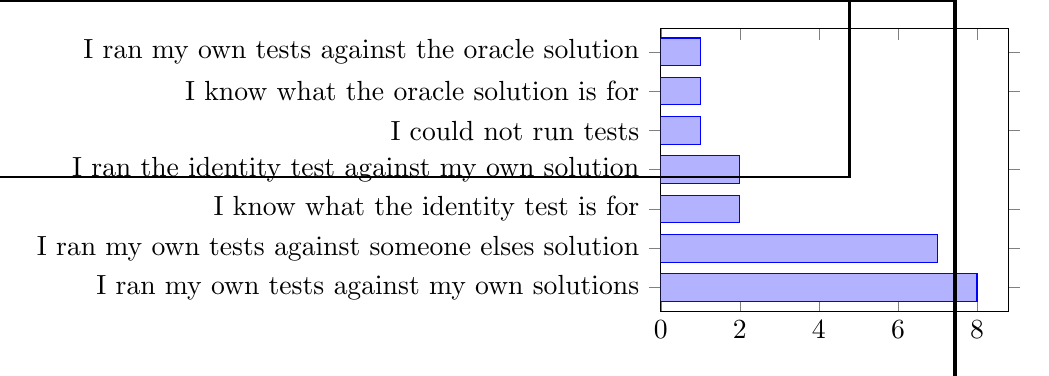
\begin{tikzpicture}
\begin{axis}[
xbar, xmin=0,
width=6cm,
symbolic y coords={I ran my own tests against my own solutions,I ran my own tests against someone elses solution,I know what the identity test is for,I ran the identity test against my own solution,I could not run tests,I know what the oracle solution is for,I ran my own tests against the oracle solution},
ytick=data,
]
\addplot coordinates {(8,I ran my own tests against my own solutions) (7,I ran my own tests against someone elses solution) (2,I know what the identity test is for) (2,I ran the identity test against my own solution) (1,I could not run tests) (1,I know what the oracle solution is for) (1,I ran my own tests against the oracle solution)};
\end{axis}
\end{tikzpicture}
\caption{Question asked users to select all statements that applied to them}
\label{fig:stmt-test}
\end{figure}
When asked about the testing functions used on the site, 8 / 11 respondents tested their own solution and 7/11 said they felt they had tested someone elses solution. As part of the feedback process all of them would have had to test the other persons solution, but this was done automatically, so it may not have been entirely clear what was happening. Similarly, comparatively few people used the identity\footnote{At this point, the test I was using to check the interfaces matched up was called the identity test. I decided to change it to something more meaningful - the Signature test, and this is the nomenclature used throughout the rest of this document.} test and oracle tests. This suggests that these also need better explanation. In the discussion session, one participant said they liked having a good working solution they could test against, so it would be worth emphasising the existence of these options more.\par
Further to this, when asked for a detailed explanation of any other problems with the site, One respondent said that the flow of the website when running tests was somewhat disrupted - When running tests you are shown a message saying the test is being run, but there is no indication of what to do next. Once tests are complete or files uploaded, you are left with many nonsensical IDs and these are hard to read and work with.
\subsection{Permission Issues}
\label{sec:permiss}
This iteration of the site allowed an uploaded submission to be marked as private. In retrospect I do not think this is a particularly useful feature, as regardless of private values, only the solution marked as final will be shared, and anything else is hidden. The inclusion of this setting likely caused some confusion, which resulted in some files not being usable when a tester goes to give feedback.
\subsection{Feedback}
One issue that cropped up in both the survey, and I was contacted directly by a participant over, was that once a feedback comment has been submitted for a test match, it cannot be modified. This caused issues for one participant as they had accidentally clicked the submit button. It may be worth modifying this such that feedback can be changed after it has been submitted, although a history of responses would need to be kept.\par
\subsection{Site Appearance and Layout}
There are many usability issues in the website. Partly stemming from the lack of nice appearance and layout, which might act psychologically to make people think its more complicated. The UX of the site is also poor. There are issues with explanation of features available and general understanding of what each part of the site does (with the exception of the feedback view, which was found to be self-explanatory, once participants were able to find it).\par
The layout of the feedback view was good, with praise for the automatic syntax colouring of the code. However, it was suggested that the tab view could become harder to navigate if there were many files as there was little distinction between the different types of file (such as source code, test results, etc.).\par
\subsection{Device Usage}
Regarding the performance of the website on different devices, while participants were not instructed in which device type to use, I felt it worthwhile to ask anyway. All of the participants responded saying the used a desktop/laptop device. This is also the same type of device they normally do development of code on, although 1 respondent did say they also used a tablet computer, and 1 said they used a mobile device to program. When asked about what would be a use case for the website and mobile devices, 6 respondents said that they would use either tablet or mobile devices to interact with the feedback view. This same point was agreed upon in the discussion session.\par
\subsection{Teacher View}
Although it was not tested by the evaluation study participants, during the study I took on the role of a teacher who would manage the simulated coursework exercises through the teacher view of the website.\par
The teachers view was created with quite minimal functionality, with most focus given to the student view. This did cause some issues though, for example with regards to editing descriptor files for a given coursework - this is simply not supported and would of course be an addition that would be needed for actual use by a teacher. As previously mentioned, the way the website uses random identifiers for files made it somewhat confusing at times.

\section{Speed}
\textit{Did the website allow for a faster turnaround of feedback than other methods?}\par
\subsection{Timing}
Looking at the times between when the solution was sent / made available to the other person, I was able to analyse the difference between when the time the feedback was received. Ideally, this would be as low as possible.
\begin{figure}[ht]
\centering
\begin{tabular}{l||r|r}
 & \textbf{Email} & \textbf{Website}\\
\hline
\textit{Avg} & 26.31 & 18.17 \\
\textit{Min} & 6.50 & 0.68 \\
\textit{Max} & 43.02 & 44.53 \\
\textit{Samples} & 4 & 9 \\
\end{tabular}
\caption{The time difference between making solutions available and receiving feedback (Hours)}
\label{tab:timing}
\end{figure}
This data in figure \ref{tab:timing} shows that the website seems to have, on average, a lower wait to receive feedback. It did however, end up having a larger wait time in the worst case. However, the total number of samples I was able to get was lower than I would have expected, so this data may not be entirely representative of the reality.
\subsection{Participant Opinions}
During the discussion session, a question was asked about how the site fared compared to running tests on the command line. The point was made that the website was ``helpful in automating running the tests'', but that it was ``not as quick as bashing something out on the command line''. This would suggest that it may be faster for testers to download file and tinker with them before running their own command line actions. A suggestion was made that a built-in editor could be made to allow either the developers or the testers to modify files, as this would be faster than editing on a computer and having to re-upload them.\par
Some participants suggested that the ability to receive notifications via email when new feedback was available would be useful, and this would certainly increase the turnaround time for feedback being sent through the website.\par
A student from Edinburgh noted that in other Non-anonymous paired exercises, such as pair programming, things can be slowed down as you may choose to not give some feedback for fear of hurting feelings. Therefore, a site that offers anonymity should help to provide a safe space for feedback.

\section{Enhance}
\textit{Did the website improve the level of feedback given?}\par
It is important that if the website works properly, that the feedback and learning that happens as a result of using it is useful. Ideally it would outperform other means of peer-testing feedback and learning. Due to the issues that occurred with many tests not running fully, I feel that the feedback given on the site would obviously not be as detailed as one would expect.\par
\subsection{Cross-Campus Learning}
One of the benefits that using a website would offer is that it could make it easier for peer-testing activities to take place across campuses. During the discussion session, when the participants were asked about their opinions on cross-campus learning such as this, they felt that it was much more ``interesting''. Within the feedback,  there is greater scope for learning across campuses as you can give feedback based on different experiences you have had learning, and the different ways that lecturers will teach across campuses.
\subsection{Unit-Testing}
During the discussion, a point was raised about how people normally do testing. Some said that they did not always to formal testing, but informally tested their code as it was developed. One participant said that by forcing themselves to write the unit tests this time, something they did not normally do, it revealed shortcomings in their own code that they had missed. This would suggest that the way the site forces the students to write code is beneficial.
\subsection{Peer Activities}
In order to find out students perceptions of peer activities, I asked if any had completed some before. Only 2 respondents to the survey had prior experience in peer activities. The peer activities were ``Essay peer-marking, giving feedback'' and ``Checking correctness and logic of code of other students in high school''. These responses would seem to suggest that peer activities are not currently utilised very much in programming courses at university.\par
The participants were asked to rate their opinions on whether or not they agreed with certain website and peer-testing related statements. In figure \ref{tab:peer-test} the results can be seen.\\
\begin{figure}[ht]
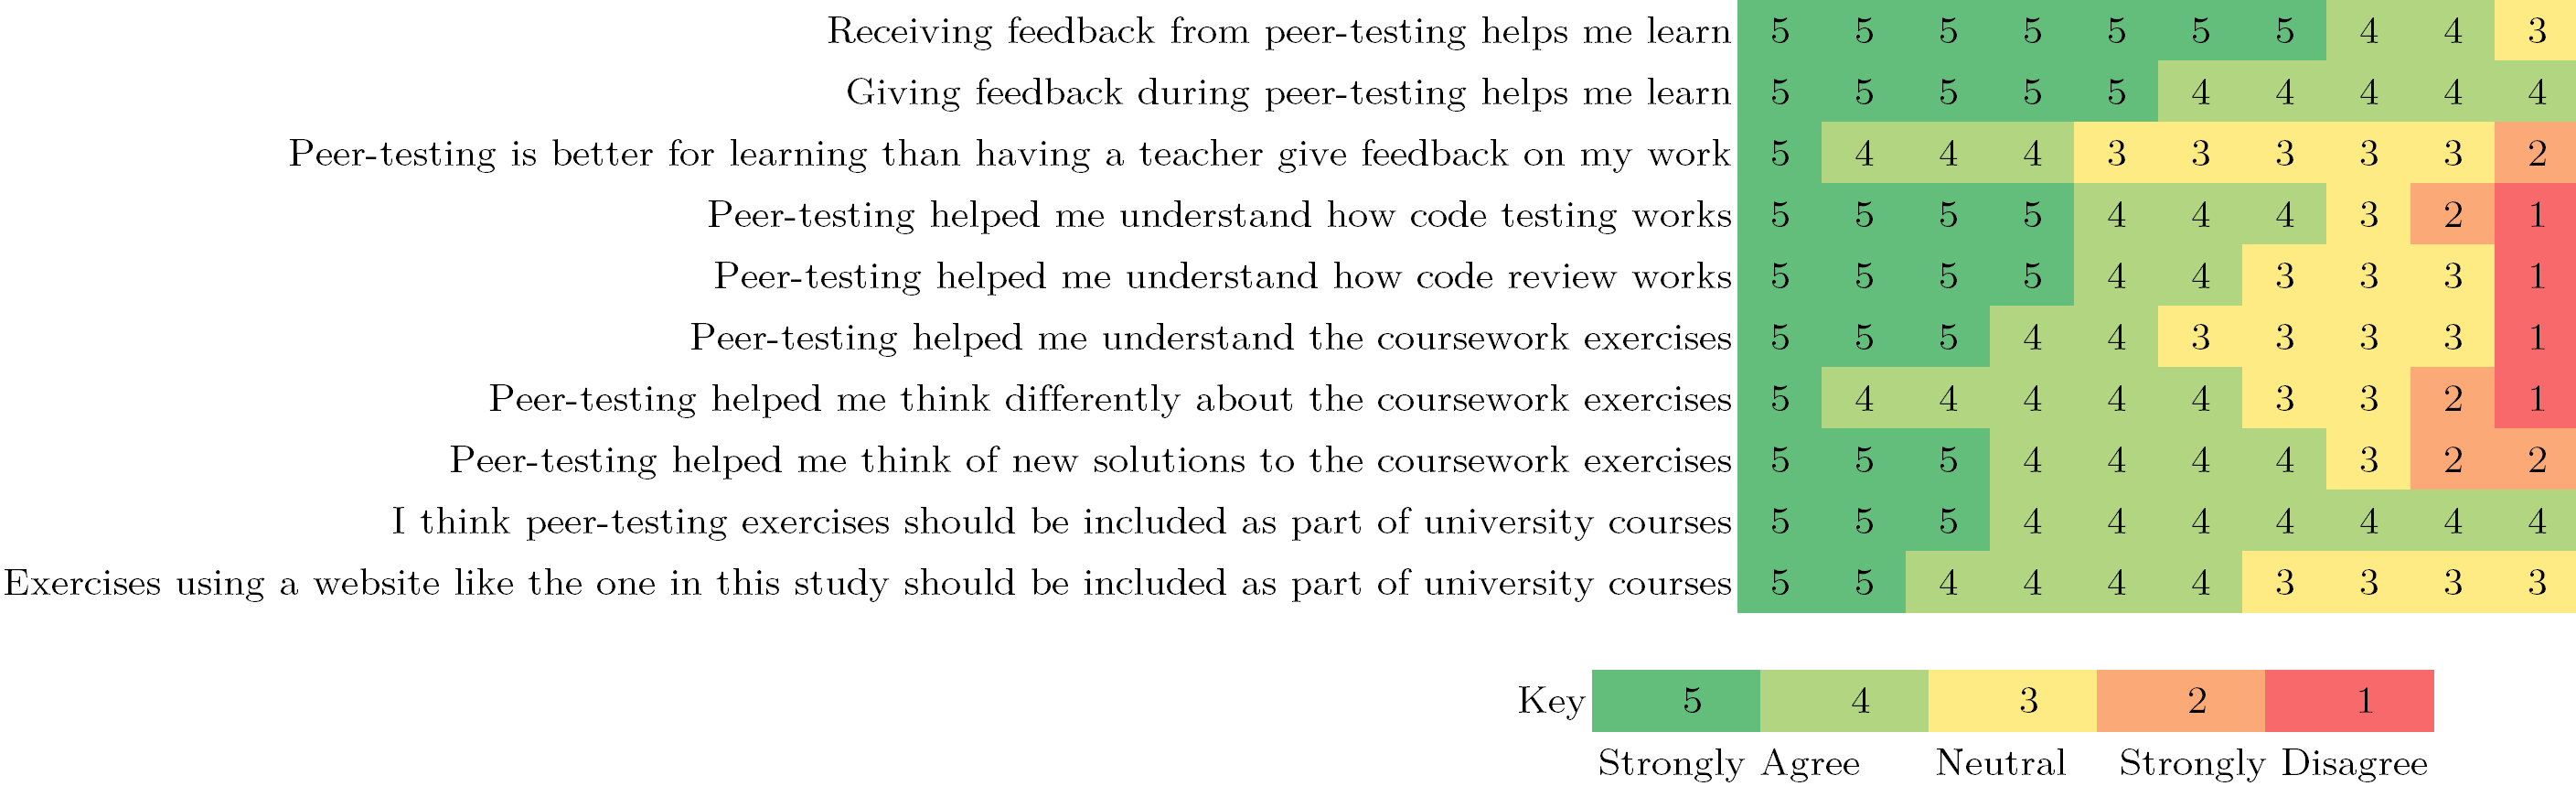
\includegraphics[width=\textwidth]{eva-result/likert-peer-test.png}
\caption{Responses for Likert questions with regards to peer-testing and the website}
\label{tab:peer-test}
\end{figure}\par
\tiny
\begin{tabular}{r|cccccccccccc}
Receiving feedback from peer-testing helps me learn & \cellcolor{Green} 5   & \cellcolor{Green} 5   & \cellcolor{Green} 5   & \cellcolor{Green} 5   & \cellcolor{Green} 5   & \cellcolor{Green} 5   & \cellcolor{Green} & \cellcolor{LimeGreen} 4   & \cellcolor{LimeGreen} 4   & \cellcolor{LimeGreen} 4   & \cellcolor{LimeGreen} 4   & \cellcolor{Goldenrod} 3 \\
Giving feedback during peer-testing helps me learn  & \cellcolor{Green} 5   & \cellcolor{Green} 5   & \cellcolor{Green} 5   & \cellcolor{Green} 5   & \cellcolor{Green} 5    & \cellcolor{LimeGreen} 4   & \cellcolor{LimeGreen} 4   & \cellcolor{LimeGreen} 4   & \cellcolor{LimeGreen} 4   & \cellcolor{LimeGreen} 4   & \cellcolor{LimeGreen} 4\\
Peer-testing is better for learning than having a teacher give feedback on my work  & \cellcolor{Green} 5    & \cellcolor{LimeGreen} 4   & \cellcolor{LimeGreen} 4   & \cellcolor{LimeGreen} 4   & \cellcolor{Goldenrod} 3   & \cellcolor{Goldenrod} 3   & \cellcolor{Goldenrod} 3   & \cellcolor{Goldenrod} 3   & \cellcolor{Goldenrod} 3   & \cellcolor{YellowOrange} 2    & \cellcolor{YellowOrange} 2\\
Peer-testing helped me understand how code testing works    & \cellcolor{Green} 5   & \cellcolor{Green} 5   & \cellcolor{Green} 5   & \cellcolor{Green} 5    & \cellcolor{LimeGreen} 4   & \cellcolor{LimeGreen} 4   & \cellcolor{LimeGreen} 4   & \cellcolor{Goldenrod} 3   & \cellcolor{Goldenrod} 3   & \cellcolor{YellowOrange} 2    & \cellcolor{RedOrange} 1\\
Peer-testing helped me understand how code review works & \cellcolor{Green} 5   & \cellcolor{Green} 5   & \cellcolor{Green} 5   & \cellcolor{Green} 5    & \cellcolor{LimeGreen} 4   & \cellcolor{LimeGreen} 4   & \cellcolor{Goldenrod} 3   & \cellcolor{Goldenrod} 3   & \cellcolor{Goldenrod} 3   & \cellcolor{Goldenrod} 3   & \cellcolor{RedOrange} 1\\
Peer-testing helped me understand the coursework exercises  & \cellcolor{Green} 5   & \cellcolor{Green} 5   & \cellcolor{Green} 5    & \cellcolor{LimeGreen} 4   & \cellcolor{LimeGreen} 4   & \cellcolor{Goldenrod} 3   & \cellcolor{Goldenrod} 3   & \cellcolor{Goldenrod} 3   & \cellcolor{Goldenrod} 3   & \cellcolor{Goldenrod} 3   & \cellcolor{RedOrange} 1\\
Peer-testing helped me think differently about the coursework exercises & \cellcolor{Green} 5    & \cellcolor{LimeGreen} 4   & \cellcolor{LimeGreen} 4   & \cellcolor{LimeGreen} 4   & \cellcolor{LimeGreen} 4   & \cellcolor{LimeGreen} 4   & \cellcolor{Goldenrod} 3   & \cellcolor{Goldenrod} 3   & \cellcolor{YellowOrange} 2    & \cellcolor{YellowOrange} 2    & \cellcolor{RedOrange} 1\\
Peer-testing helped me think of new solutions to the coursework exercises   & \cellcolor{Green} 5   & \cellcolor{Green} 5   & \cellcolor{Green} 5    & \cellcolor{LimeGreen} 4   & \cellcolor{LimeGreen} 4   & \cellcolor{LimeGreen} 4   & \cellcolor{LimeGreen} 4   & \cellcolor{Goldenrod} 3   & \cellcolor{YellowOrange} 2    & \cellcolor{YellowOrange} 2    & \cellcolor{YellowOrange} 2\\
I think peer-testing exercises should be included as part of university courses & \cellcolor{Green} 5   & \cellcolor{Green} 5   & \cellcolor{Green} 5    & \cellcolor{LimeGreen} 4   & \cellcolor{LimeGreen} 4   & \cellcolor{LimeGreen} 4   & \cellcolor{LimeGreen} 4   & \cellcolor{LimeGreen} 4   & \cellcolor{LimeGreen} 4   & \cellcolor{LimeGreen} 4   & \cellcolor{LimeGreen} 4\\
I think peer-testing exercises using a website like the one in this study should be included as part of university courses  & \cellcolor{Green} 5   & \cellcolor{Green} 5    & \cellcolor{LimeGreen} 4   & \cellcolor{LimeGreen} 4   & \cellcolor{LimeGreen} 4   & \cellcolor{LimeGreen} 4   & \cellcolor{Goldenrod} 3   & \cellcolor{Goldenrod} 3   & \cellcolor{Goldenrod} 3   & \cellcolor{Goldenrod} 3   & \cellcolor{YellowOrange} 2\\
\end{tabular}
\normalsize

It is reassuring to see that the results affirm the previous research into this area \S\ref{sec:peer-test-why}, suggesting that students believe they learn more by giving feedback as opposed to receiving it. There seems to be a somewhat mixed response to the idea that peer-testing can be better than a teacher's response, so an addition the site may benefit would be from allowing teacher interaction as well as peers. For the most part, it seems that students respond positively that the peer-testing helps with completing the exercises, and that this should be encourage in the university. Interestingly, the response to using such a peer-testing website more in university was less positive. This may be an indicator that the participants did not find the website all that useful.\par
Having had some experience with the site, I asked the participants in the discussion if they felt there were any courses or activities within courses they felt would be improved by using the peer-testing feedback offered by the website. They suggested that the website would be useful for
\begin{itemize}
\item Larger Courseworks, which are likely to have very different solutions thus offering more places for discussion
\item Data Structures and algorithms, where there are specific assignments that fit well with the website (although they did not name any specifically)
\item Any programming exercise where the interface and specification is clearly set out
\end{itemize}
One concern was raised however in that offering such peer-testing might be detrimental to completing some exercises as it opens up a surface for plagiarism\footnote{This was a concern initially, hence why the website operates with two modes, requiring solutions to be uploaded before feedback is given.}. But in contrast, the point was made that there is a big difference in allowing such feedback to be given before the final submission deadline, as it would allow you to improve your code based on the feedback given. A suggested middle-ground was that there be three deadlines for a coursework - one for the submission of a solution, one for giving feedback, an done for suggesting how code would be fixed based on that feedback; where the overall grading for the coursework took stock of each point of participation.\par
Having looked at some of the email based feedback, it looked as though many of the students were also providing feedback on the test cases themselves, in addition to the solution. It may be worth changing the way the website works to allow this sort of feedback also, as that may provide for more avenues for learning about how to improve both solutions and tests.\par
Also, discussion noted that when you are giving feedback to a person, it is much more direct and that you can share ``insider knowledge'' of shortcuts in programming through discussion and feedback.\par
\subsection{Anonymity}
The question of anonymity was important in this website, and in the discussion session this point was reinforced by many. Some survey questions involved checking if the participants were able to guess who they were giving feedback to on the website. Only 1 responded with a maybe, and 1 yes when asked if they knew who wrote the code they were testing. When asked if they knew the location of the person whose code they were testing, 3 said they knew, 1 maybe knew the location. Of course, there was no way to be sure about this \footnote{In retrospect, it would have been useful to ask this an open-answer field so I could confirm responses}. The low number of positive guesses as to who others were suggests that the site does offer anonymity.\par
A participant mentioned that peer discussions done previous on the university VLE discussion boards would have been improved had the discussion been completed anonymously. The site currently offers anonymous feedback but doesn't yet allow for a multi-way discussion, but this comment suggests that it would fit in well. The point was raised that anonymity is better as it ``reduces judgements'' on people, and thus more of a focus is on the result of the exercise itself.
\subsection{Feedback}
In the discussion session, someone brought up the Idea that a 2-way discussion would be beneficial to giving more feedback. If a forum-style discussion was implemented for feedback, this could allow for feedback comments to be modified after they were sent. Another feature that seemed to have some support from participants was the concept of using inline code comments for feedback.\par
One student suggested that it would be nice to see a criteria for giving feedback (the concept of criteria-based marking was used in the cap system, see fig \ref{fig:cap}). And another participant discussed the idea that because of anonymity it may be hard to tailor feedback to the other person, so having a small amount of background information, such as their course or their programming strengths would be useful in helping to provide more relevant feedback. To complement that, one student liked the idea of having an identity in the email-based feedback as it allowed them to ``put a face to the code'' they were testing.\par

\section{Security}
\textit{Did the website act in a secure manner. Were there any security flaws?}\par
The evaluation study participants were not asked to assess the security of the website. Instead, I offer my own evaluation based on the current state of development of the prototype website.\par
At this stage, the only security in place lies within making sure users are authenticated. This would only allow university students to gain access to the system and upload / readfiles. However, due to a lack of time before the evaluation took place, I was unable to complete some of the other security features previously discussed.\par
The user authentication works very well. Once a user account is created, the user is assigned a group -- either teacher or student, and this is checked along with the user credentials when accessing any views through python decorators. Using these ensures that only the correct type of user can access various parts of the system. It is possible in certain cases that the checking of permissions of which users can view which files is too restrictive.\par
One issue I noticed lies with the way I handle the error output from having run the test cases. Firstly, the error output does not properly hide the file paths, which reveals information about the internals of the application (such as directories), and the output is not bounded by length. One student created a test case that failed due to a recursion limit. As a result, a very large stack trace was produced, and subsequently stored in a text file. This could pose a problem if there were many large files being created, as the website wold run out of storage. Similarly, there is no restriction on the maximum filesize the user can upload.\par
There is also little restriction in this iteration of the website when considering what kind of scripts the user may run. Currently any python script can have access to any file uploaded, and potentially a user could upload any sort of script + a python script and have the python script call that other script. Scripts are also currently run on the same level as the website application itself, rather than as a user, which could lead to scripts being run in too permissive a fashion.

\section{Summary}
\subsection{Correctness}
Many of the issues with tests failing were not due to the site. Upon closer inspection, many of the failed tests were due to the way that either the tests or the solution code was written. The only real way to reduce the number of failing tests would be to better explain how the website will run the tests. Issues with files not being readable were again due to a lack of explanation as to how that feature worked.
\subsection{Usability}
This evaluation study revealed many issues with the usability of the website. The main design of the website, and the lack of clear explanation as to how it would function caused some confusion in both how to use the website, and how the various features that were available fit together. This in turn resulted in requiring a lot of effort on the part of the users to get the functionality working right. To correct these issues, I would propose the following changes to the site, or considerations for the future:
\begin{itemize}
\item Add some in-place / contextual help tips to better explain what each part of the site is supposed to do
\item Remove the ability to mark uploads as ``private'' - this doesn't serve any purpose and leads to confusion
\item Rework the way that multiple submissions are used - possibly hide old ones and keep the latest, and stop using random file IDs on user-facing parts of the site
\item To correct indentation problems, complete support for pipelining the uploaded files, possibly making calls to re-indent\footnote{reindent.py is a module included in python that normalises the indentation to spaces only}
\item Improve the general design of the website. If it looks better, people will feel more comfortable using it
\item In the feedback view, make explicit what each file is from - i.e. if it is a solution source code, a test result etc.
\item To prevent confusion when a user is running their own test case, make the page they are directed to fit in more with the site, and include an explanation of how the testing is done. Then automatically redirect them to the results when it is complete.
\item Test that the feedback view works well with mobile devices
\item Re-design the way that interactions with the website are reported through the teacher view
\end{itemize}
\subsection{Speed}
The evidence I was able to collect did suggest that the website offers for a faster turnaround than a peer exercises that uses e-mail as a base. Further investigation of this, with larger numbers, might be required to say with certainty. Suggested features to improve turnaround time even more included E-mail notifications for any new feedback, and a built-in editor to allow for quick tweaking of code for testing.
\subsection{Enhance}
The website did seem to make some steps towards providing better feedback and learning. The way the website operates allows for cross-campus activity and forces students to make use of unit-testing. Both of these features help enhance the learning and feedback that occurs during the process. Students felt that peer activities would be welcome if they were used in university courses more, and that the website would work well with Large courseworks in courses such as Data Structures \& Algorithms where the courseworks have clearly laid out specifications. Praise was given for the anonymity offered by the website as this allowed for more open feedback.\par
One change that was discussed would be to introduce a way of allowing for multi-way discussions for feedback, in place of the current single-comment-per-test. This would allow for better communication and discussion of results and allow for more learning and sharing of insights into the code.
\subsection{Security}
The security in terms of authentication on the website is very good, and I believe there are sufficient checks to make sure that only the right users are able to use the right parts of the website. However, once these users are logged in, they are given too much trust that they will not abuse the system. The output that they are given from the website having run tests should be stripped down, possibly as part of piping the output of the tests and making sure that any directories are removed

%more stuff...
Add more pipelining - possibly checks for filesize, process of results.txt to remove sensitive info Manuel made a suggestion at an earlier stage about using the filesystem directly instead of models - perhaps if i'm going to implement pipelines properly then I could simply forego the models for FILE. Because if I have the information from the submission model, that's enough to build up the file system\par
% END


% CONCLUDE
% BEGIN
\chapter{Conclusion}
\section{Achievements}
what I have achieved according to objectives, and prior work done in the area
the main limitations
\section{Future work}
Discuss possible additions to allow this to be used within an actual learning context.\par
Some initial testing with the concept of WebSocket-based notifications was done at this stage, and a basic proof of concept showed that notifications could be used. However, this was not as simple as plugging in a module, as some changes to the base configuration of the Django application was needed. Therefore, to ease development of the prototype, the concept of the notifications was removed for later implementation.\todo{right place to put this?}\par
% END



% APPENDICES AND BIBLIOGRAPHY

\pagebreak
\singlespacing
\printbibliography
\addcontentsline{toc}{chapter}{Appendices}

% ETHICAL
%BEGIN
\addcontentsline{toc}{section}{A: Ethical Analysis}
\section*{A: Ethical Analysis}
\label{app:ethical}
\textbf{Student}: L\'eon McGregor\\
\textbf{Title}: Web platform for code peer-testing\\
\textbf{Supervisor}: Manuel Maarek\\
\textbf{Abstract}: Develop a web platform for managing peer-testing and peer-feedback of programming code. The project aims at providing a user-friendly solution for giving and receiving feedback on programming artifacts.\\
\textbf{Purpose of Study}: The purpose of this study is to investigate the effectiveness of a prototype web platform for peer assessment of programming code. The test subjects will be asked to perform small programming exercises, and peer assess each others work. The test subjects will attempt this without and then with the prototype website, in order to see if the website is effective. Test subjects will also be given some questionnaires to fill out, and may participate in an extended discussion session if they choose.

\subsection*{Screening}
\textbf{Does the research involve any of the following?}: Human Subjects\\
\textbf{Interface Only Screening?}: No\\
\textbf{Full Ethical Screening?}: Other body not required

\subsection*{Use of Human Subjects}
\textbf{How will participants be recruited?}: Participants will ideally be students of computer science at Heriot-Watt. A general request for participants to join in will be sent out, perhaps through a university emailing list, or by posting flyers. This will be done up to a week before the study is conducted.\\
\textbf{All participants to be recruited are over 16, able to give informed consent, and have no known impediment that might affect their ability to participate in the study?}: Yes\\
\textbf{How long will participants have to decide whether to take part in the study?}: 7 Days\\
\textbf{Does the study involve actively deceiving participants?}: No\\
\textbf{Will participants be using non-standard hardware?}: No

\subsection*{Data Protection Compliance}
I confirm that, in accordance with Data Protection legislation:
\begin{itemize}
\item Indentifiable data will be stored on a secure machine with restricted access
\item Data will be anonymised before publication unless consent has been given
\item Identifiable data will only be retained for the duration of the consent granted by the participant
\item External data and systems will be used within the licence terms specified
\end{itemize}

\subsection*{Health and Safety}
I confirm that the project involves only standard IT equipment and exposes participants to no more hazards than a conventional office environment.

% END

\newpage
\addcontentsline{toc}{section}{B: Evaluation Consent Form}
% BEGIN
\label{app:consent}
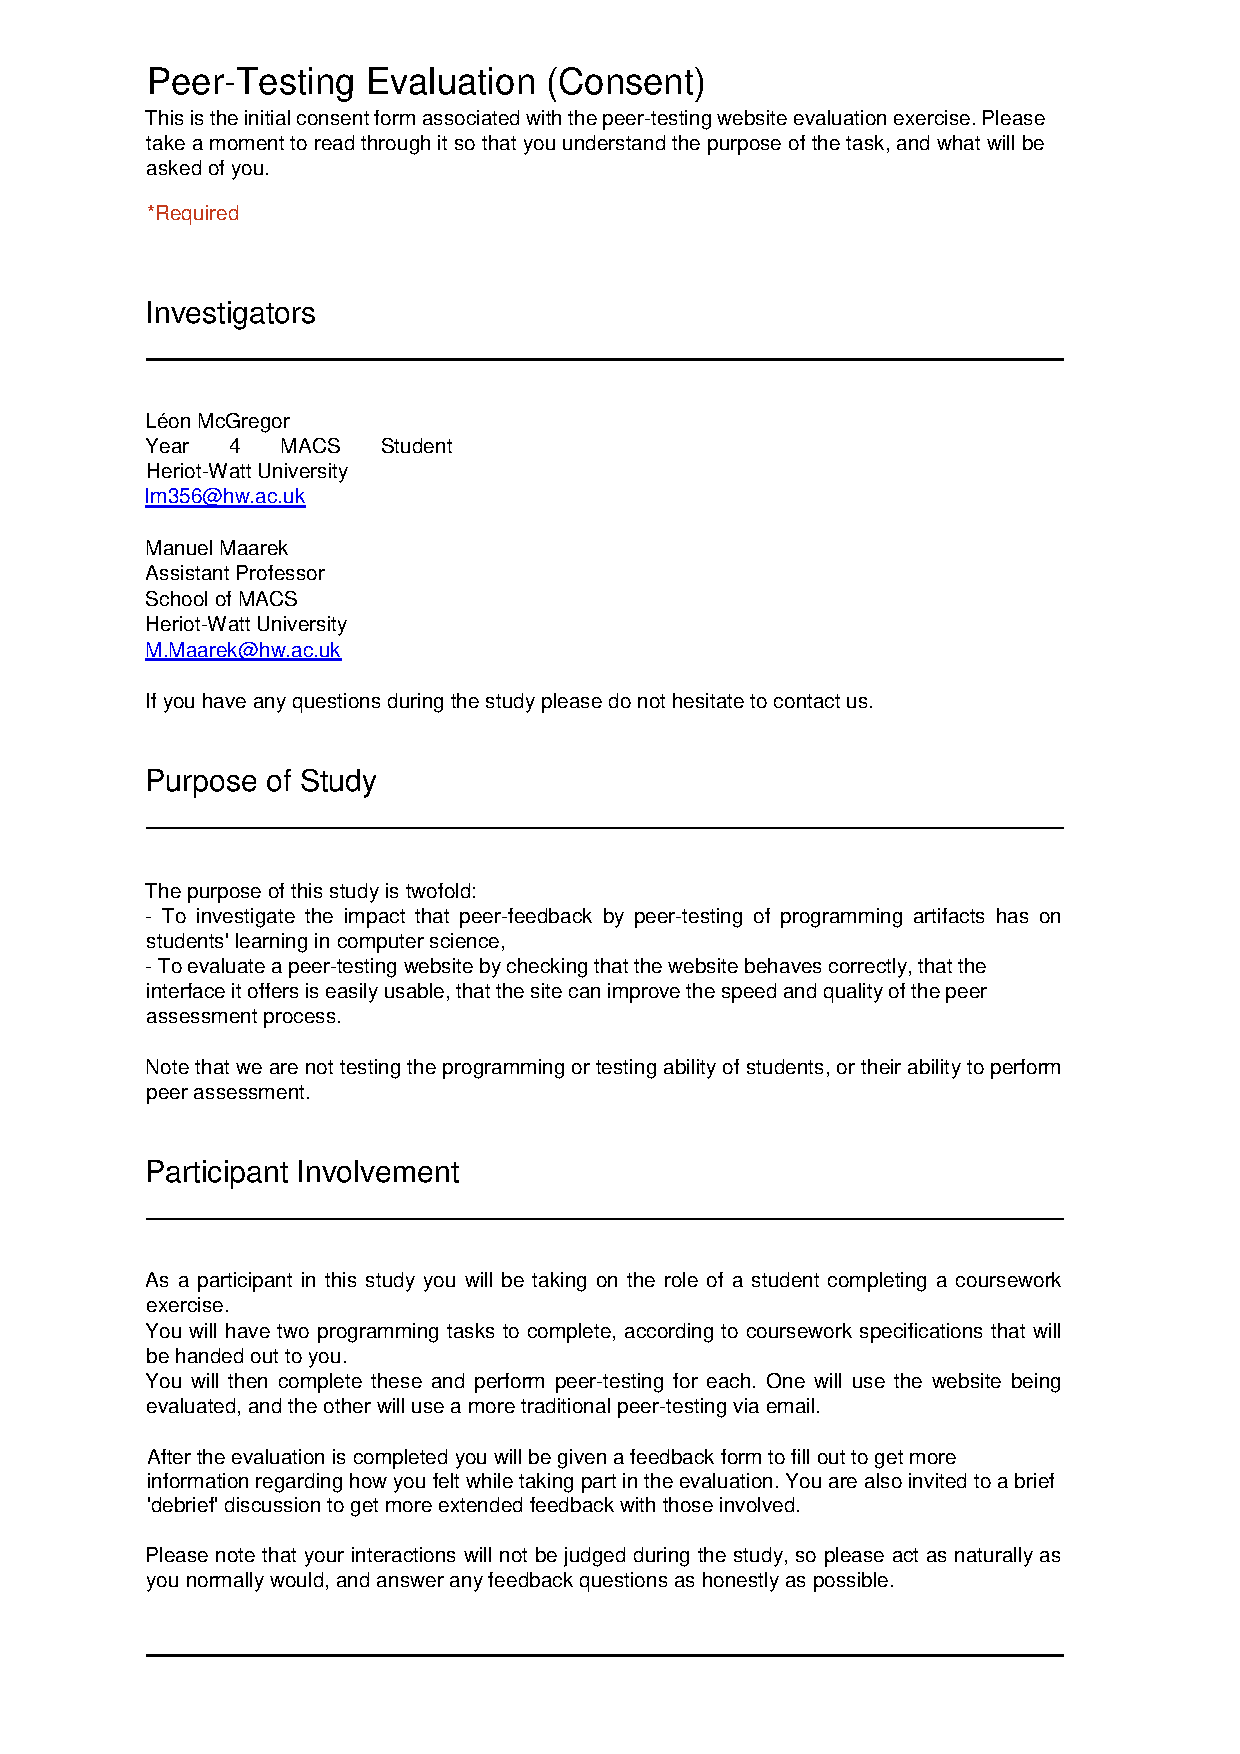
\includepdf[pages={1}]{eva/consent2.pdf}
\includepdf[pages={2}]{eva/consent2.pdf}


\newpage
\addcontentsline{toc}{section}{C: Evaluation Survey Form}
\label{app:survey}
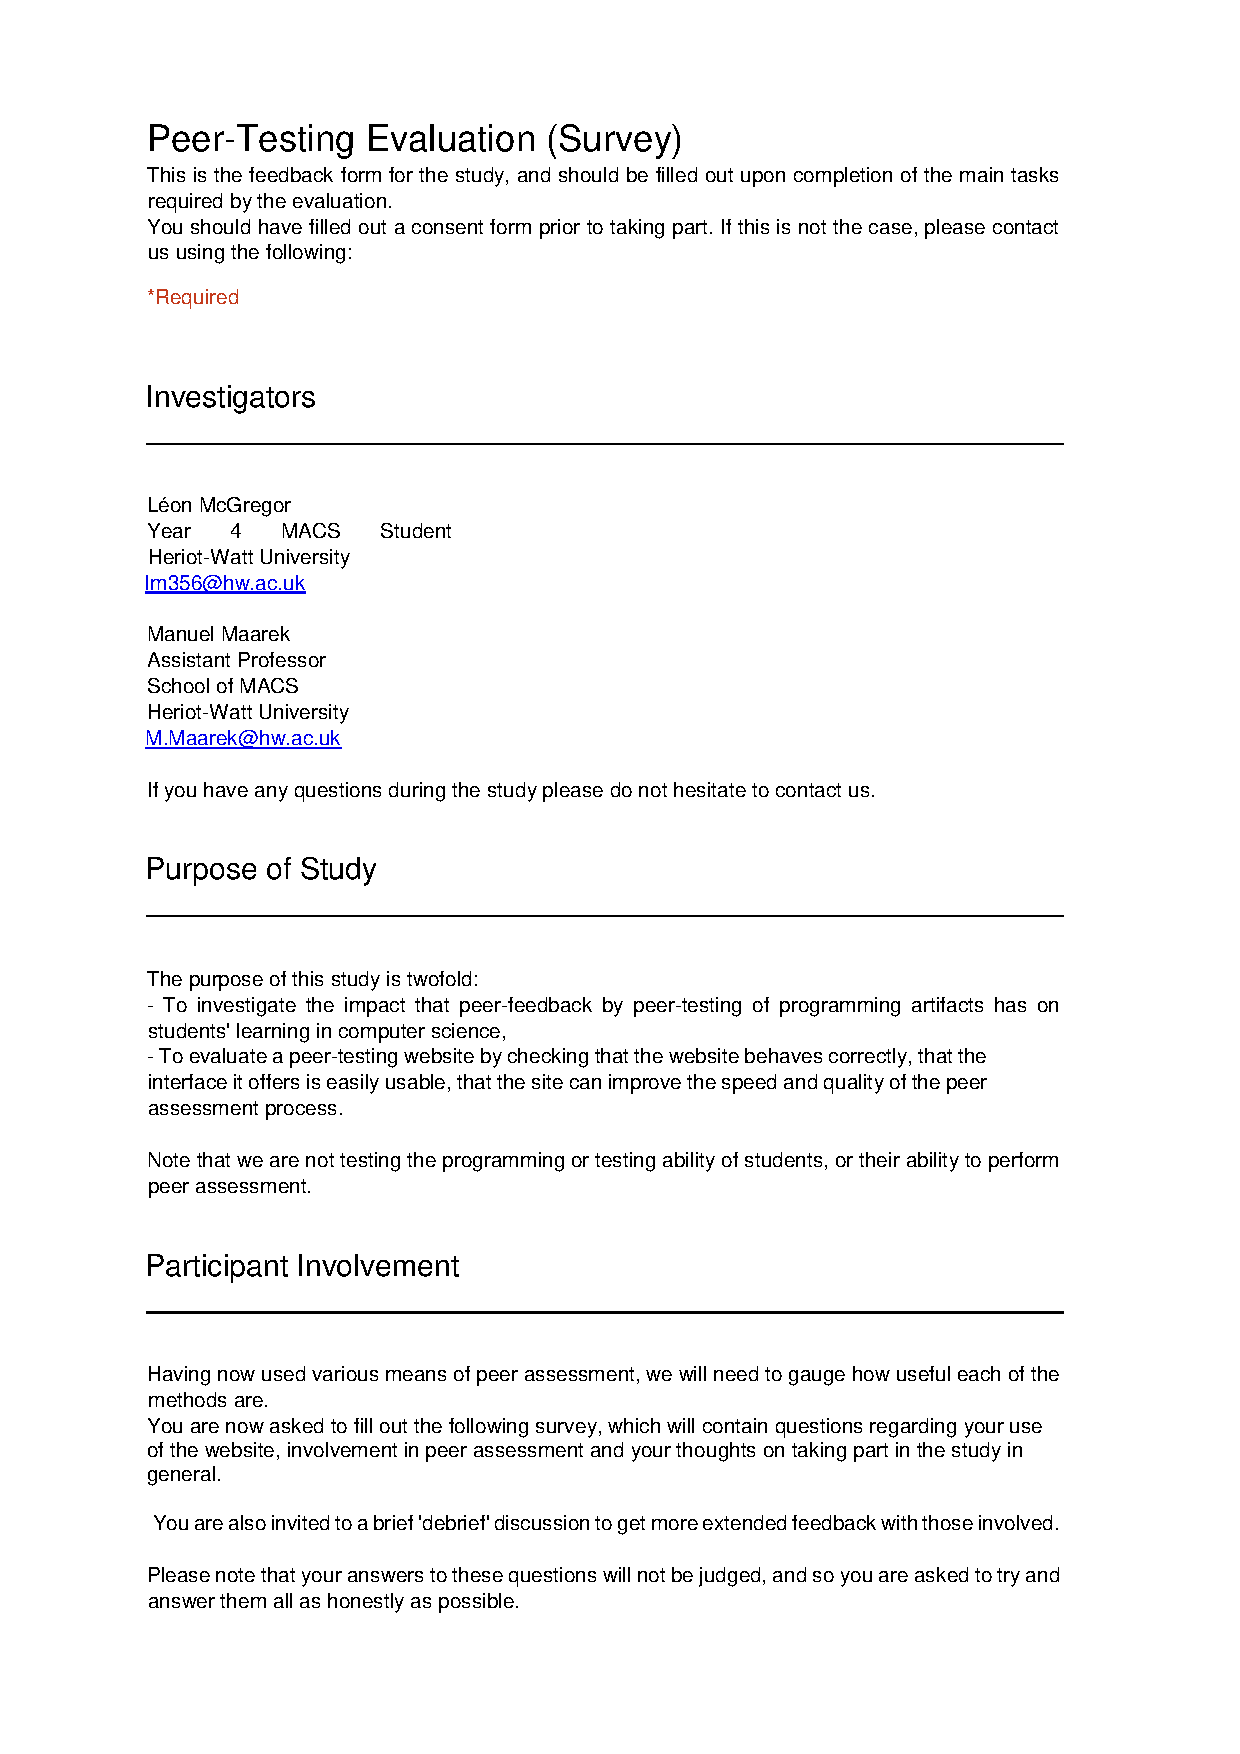
\includepdf[pages={1}]{eva/survey2.pdf}
\includepdf[pages={2}]{eva/survey2.pdf}
\includepdf[pages={3}]{eva/survey2.pdf}
\includepdf[pages={4}]{eva/survey2.pdf}
\includepdf[pages={5}]{eva/survey2.pdf}
\includepdf[pages={6}]{eva/survey2.pdf}
\includepdf[pages={7}]{eva/survey2.pdf}
\includepdf[pages={8}]{eva/survey2.pdf}
\includepdf[pages={9}]{eva/survey2.pdf}
% END


\newpage
\addcontentsline{toc}{section}{D: Evaluation Extended Discussion Questions}
 % BEGIN
\section*{D: Evaluation Extended Discussion Questions}
\label{app:discussion}
These questions were discussed in a debriefing session after the evaluation study had completed. Both Myself and Manuel Maarek had prepared some questions to ask during this evaluation study. The following were questions prepared by myself:\par
\begin{itemize}
\item Is peer feedback useful forgetting a new view on code?
\item How did you feel about running tests on the website?
\item How was running tests on the website when compared to a command line interface?
\item How do you feel about anonymity during peer activities?
\item Can you think of any classes that benefit from such a peer assessment website?
\item Can you think of any improvements that ought to be made to the website?
\item Were the exercises you completed suitable for the website?
\item In python, do you use tabs or spaces?
\item Did you enjoy taking part?
\end{itemize}
The following questions were prepared by Manuel Maarek:
\begin{itemize}
\item Do you normally write tests for your code?
\item Was it good to have time set aside for you to test code?
\item How do you feel about the feedback options afforded through peer activities or pair programming?
\item Was there enough information provided to complete the task
\item Was it clear what the website was doing behind the scenes?
\item What are your feelings on cross-campus interactions?
\end{itemize}
% END


\newpage
\addcontentsline{toc}{section}{E: Evaluation Study Task Descriptors}
% BEGIN
\section*{E: Evaluation Study Task Descriptors}
\label{app:descriptors}
What follows is a complete listing of the materials provided to the participants, who acted as students, for the study. Included is The main task descriptor, and for each coursework task (tree and quicksort):
\begin{itemize}
\item The main task descriptor
\item A empty file acting as a template that ought to be filled in
\item A signature test showing the interface that must be met
\item An empty unit test file acting as a template that ought to be filled in
\item (Not seen by students, but included here for completeness) A file containing a working solution
\end{itemize}
\newpage
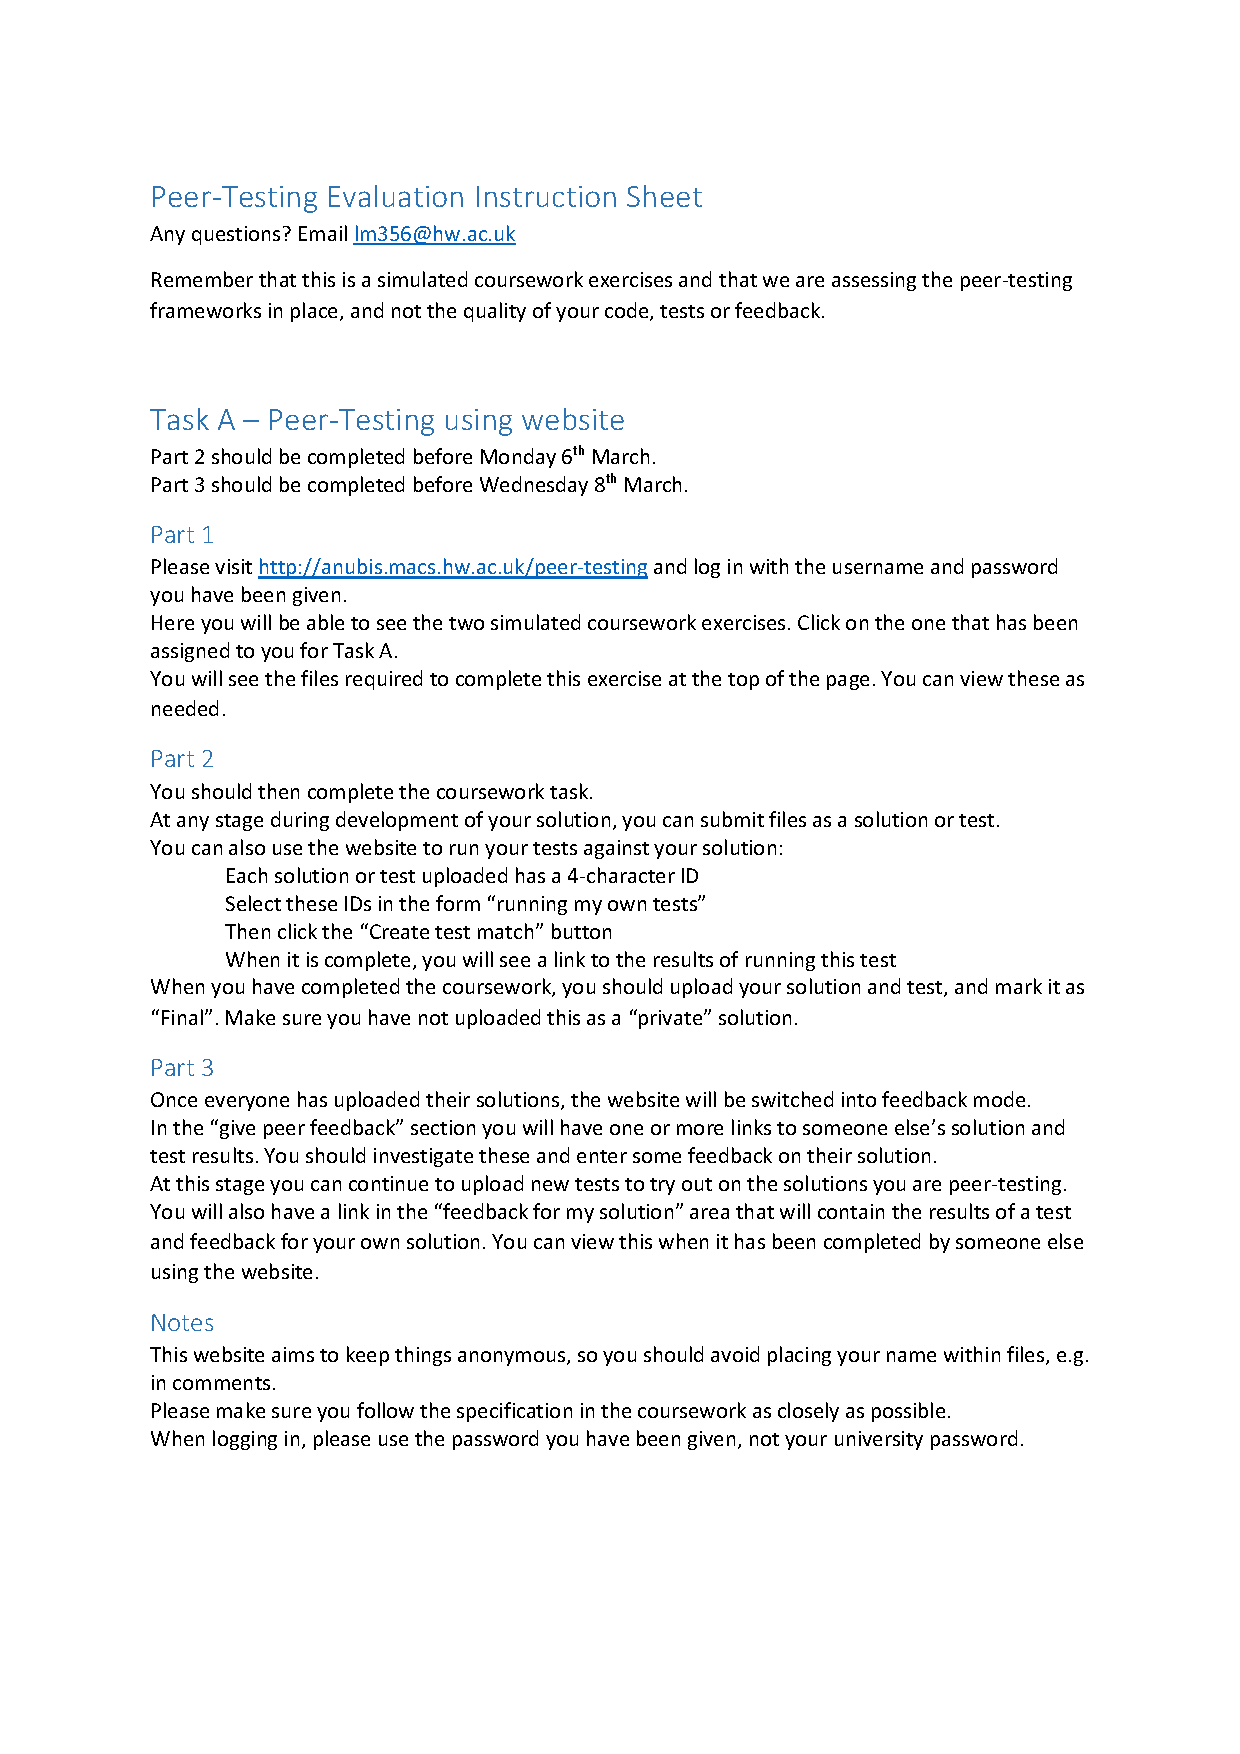
\includepdf[pages={1}]{eva/maintask.pdf}\newpage
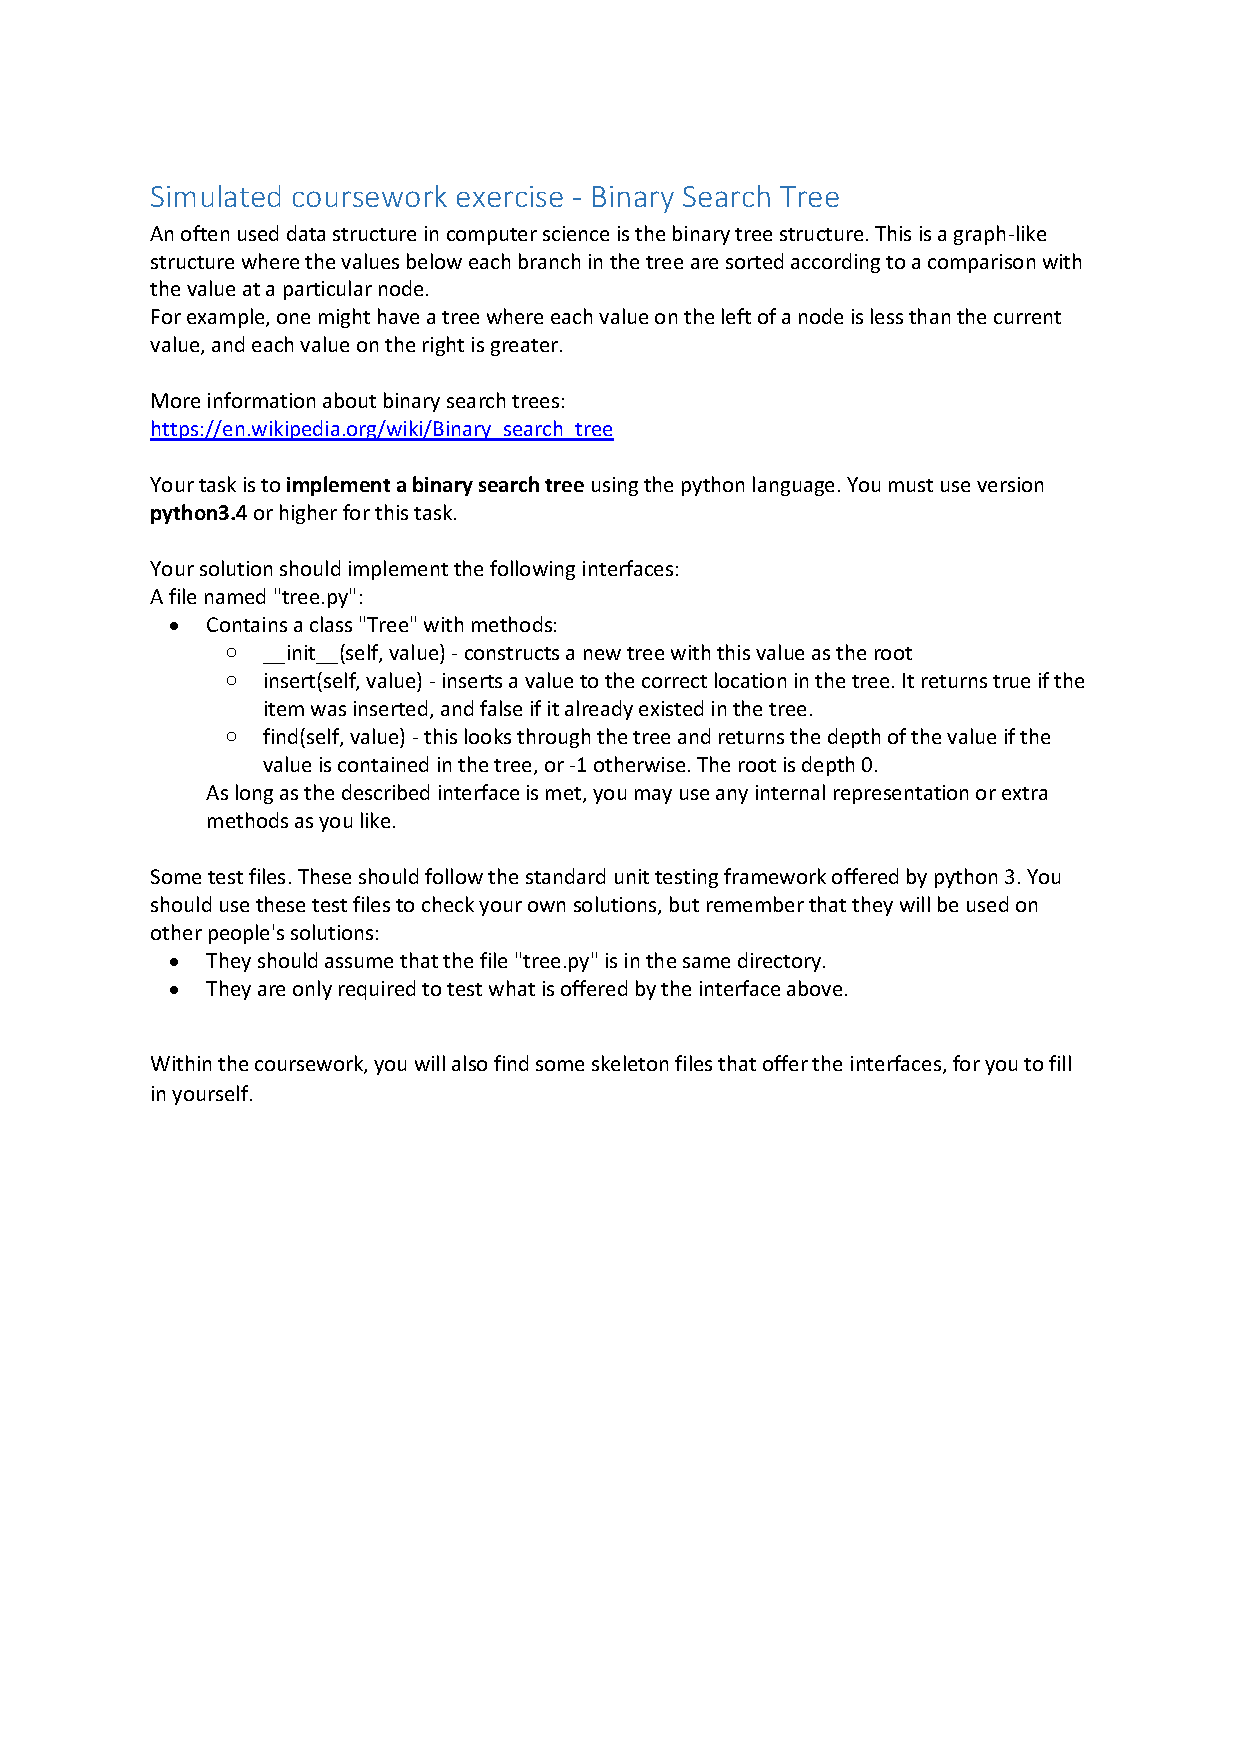
\includepdf[pages={1}]{eva/cw1/cw1-descriptor.pdf}\newpage
\lstinputlisting{eva/cw1/tree.py}\section*{}
\lstinputlisting{eva/cw1/signature.py}\section*{}
\lstinputlisting{eva/cw1/sample_test.py}\section*{}
\lstinputlisting{eva/cw1/oracle/tree.py}\newpage
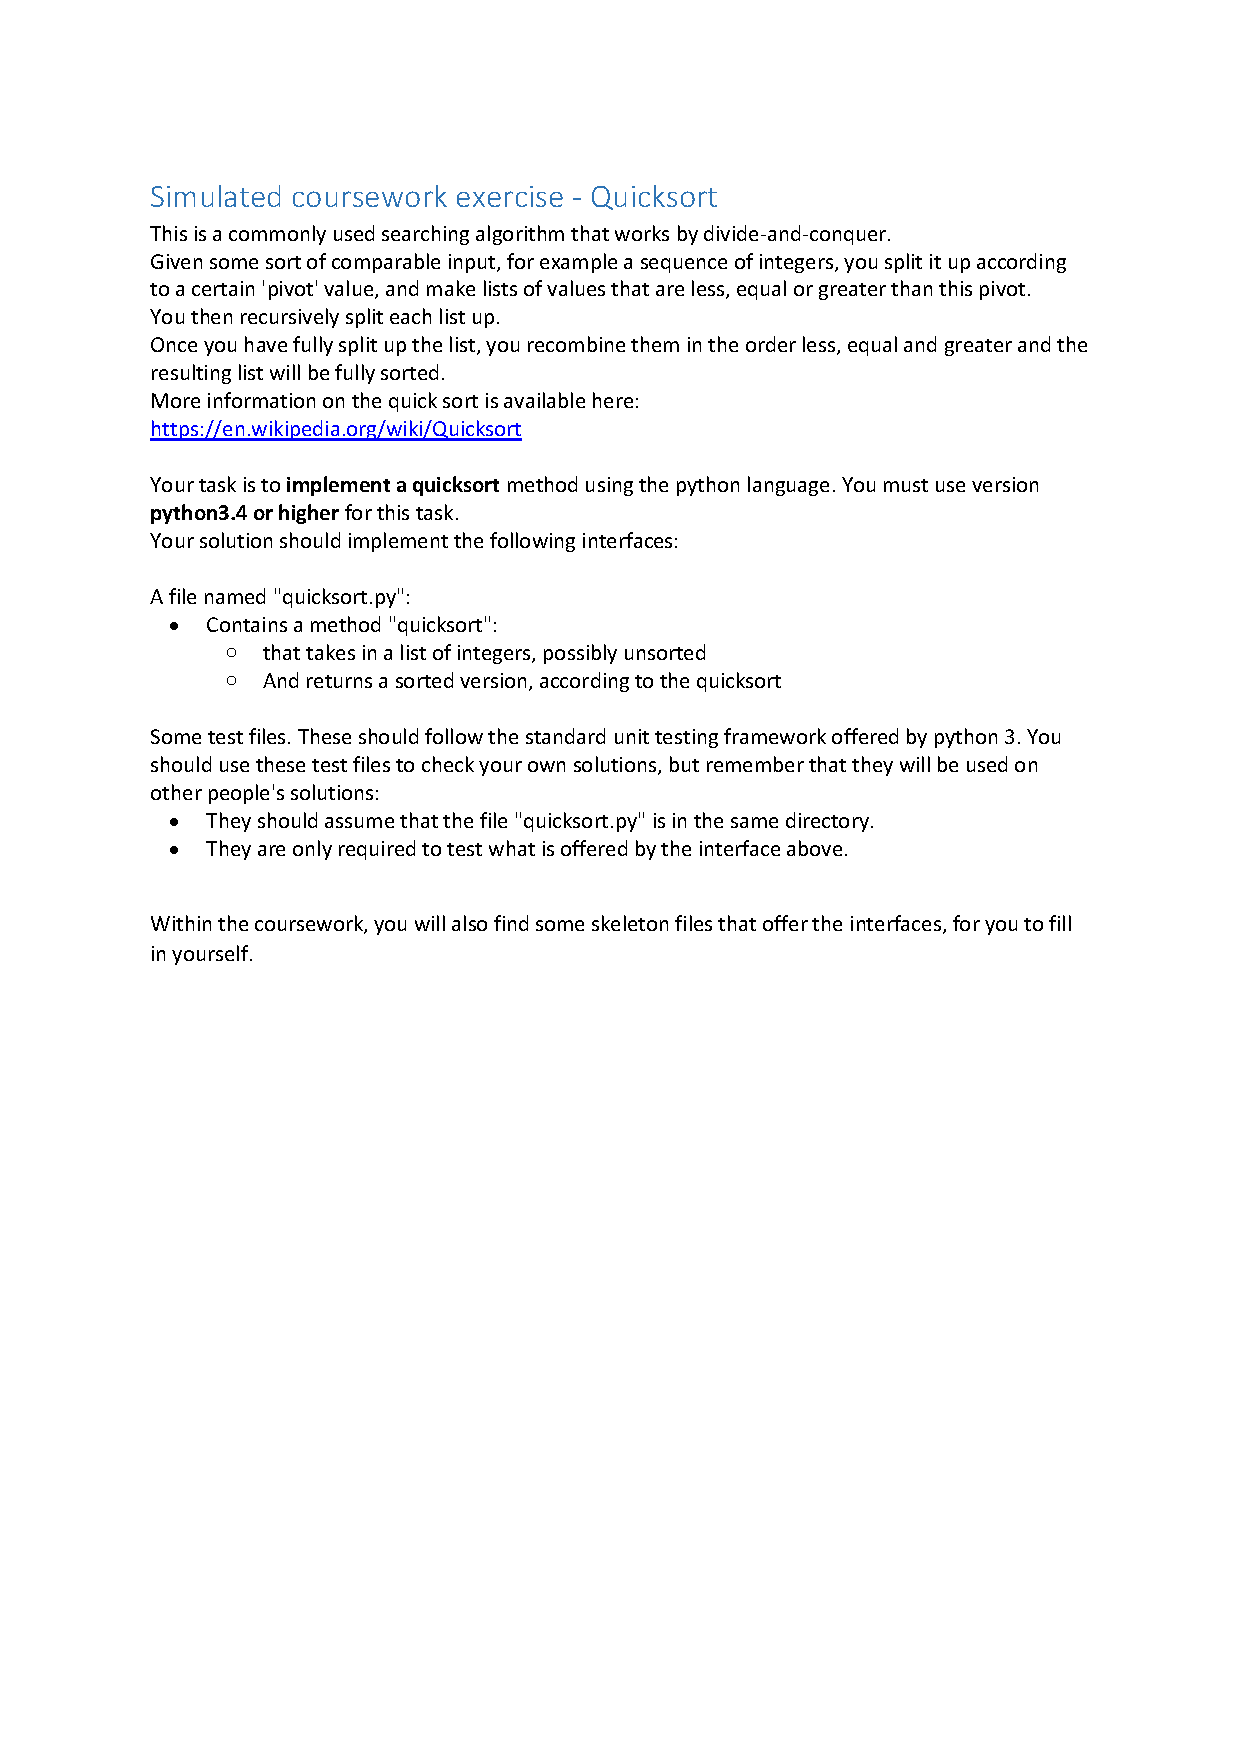
\includepdf[pages={1}]{eva/cw2/cw2-descriptor.pdf}\newpage
\lstinputlisting{eva/cw2/quicksort.py}\section*{}
\lstinputlisting{eva/cw2/signature.py}\section*{}
\lstinputlisting{eva/cw2/sample_test.py}\section*{}
\lstinputlisting{eva/cw2/oracle/quicksort.py}
% END

\end{document}